\section{Solving the OT problem for RFFs and RLFs} \label{app:rff_rlf_theory}
In this appendix, we provide proofs for the theoretical results in Sec.~\ref{sec:rffs_rlfs_theory} and supplement the discussion of copula-based numerical OT solvers in Sec.~\ref{sec:copulas}.

\subsection{Proof of Lemma \ref{lemma:ot_rff_formulation}}
We begin by proving Lemma \ref{lemma:ot_rff_formulation}, which formulates variance reduction for RFFs and RLFs as an optimal transport problem. 
We will first reason about the simpler case of RLFs, then consider RFFs.

\emph{Proof of Lemma \ref{lemma:ot_rff_formulation}}. Consider the following recently-derived result by \citet{simrfs}.

\begin{lemma}[Kernel estimator MSE for RLFs \citep{simrfs}] \label{lemma:appendix_conformity}
    When estimating the Gaussian kernel \smash{$k(\boldsymbol{x}, \boldsymbol{y}) \coloneqq \exp(- \|\boldsymbol{x} - \boldsymbol{y}\|_2^2 / 2)$} for datapoints $\{\boldsymbol{x},\boldsymbol{y}\} \subset \mathbb{R}^d$ using random Laplace features (synonymously, positive random features), the mean square error of the kernel estimate \smash{$\widehat{k}(\boldsymbol{x}, \boldsymbol{y})$} is given by:
\begin{equation} \label{eq:prf_rmse_expression}
    \textrm{MSE}(\widehat{k}) = \frac{e^{-2x^2-2y^2}}{m}\left ((e^{2v^2}- e^{v^2}) + (m-1)(\rho(\boldsymbol{x},\boldsymbol{y}) - e^{v^2}) \right)
\end{equation}
where $m$ is the number of sampled random frequencies, $v \coloneqq \|\boldsymbol{x}_i + \boldsymbol{x}_j\|_2$ is a data-dependent scalar and $\rho(\boldsymbol{x}_i,\boldsymbol{x}_j)$ is the \emph{RF-conformity}, 
\begin{equation} \label{eq:def_rf_conformity}
 \rho(\boldsymbol{x}, \boldsymbol{y}) \coloneqq
\frac{\Gamma(\frac{d}{2})}{m(m-1)} \sum_{i,j \neq i} \mathbb{E}_{\omega_{ij}}\left( \sum_{k=0}^\infty \frac{v^{2k} \omega_{ij} ^{2k}}{2^{2k} k! \Gamma(k+\frac{d}{2})} \right).
\end{equation}
Here, $\omega_{ij} \coloneqq \| \boldsymbol{\omega}_i + \boldsymbol{\omega}_j \|_2$ is the norm of the resultant of a pair of distinct frequencies and $\Gamma$ is the Gamma function. 
\end{lemma}
\emph{Proof.} \citet{simrfs}. \qed

The simple derivation, reported in full by \citet{simrfs}, is based on rewriting the angular integral as a Hankel transform, yielding a Bessel function of the first kind with a known Taylor expansion. 

%Evidently, the RF confirmity $\rho$ is the object of central interest to be suppressed by an effective coupling scheme. 
%Our strategy is induce correlations between $\boldsymbol{\omega}_i$ and $\boldsymbol{\omega}_j$ to manipulate the distribution over $\omega_{ij} \coloneqq \| \boldsymbol{\omega}_i + \boldsymbol{\omega}_j \|_2$, subject to the constraint that both frequencies must obey marginal Gaussian distributions.

Supposing that \smash{$\boldsymbol{\omega}_i \perp \boldsymbol{\omega}_j$}, we have that \smash{$\omega_{ij} = \sqrt{\omega_i^2 + \omega_j^2}$}, where $\omega_i \coloneqq \|\boldsymbol{\omega}_i\|_2$ denotes the $L_2$-norm of the frequency $\boldsymbol{\omega}_i$.
Note that, for $\boldsymbol{\omega}_i$ to be marginally Gaussian, we require that the marginal distribution over its \emph{norm} is $\chi_d$, a Chi distribution with $d$ degrees of freedom.
Substituting this into Eq.~\ref{eq:prf_rmse_expression} and dropping terms unmodified by the coupling and irrelevant multiplicative factors, it is straightforward to arrive at the expression for the cost function $c_\textrm{RLF}$ in Eq.~\ref{eq:cost_functions}. 

Finding the cost function for RFFs is only slightly more difficult. 
We begin by citing another recent result by \citet{simrfs}. 

\begin{lemma}[Kernel estimator MSE for RFFs \citep{simrfs}]
When estimating the Gaussian kernel $k(\boldsymbol{x}, \boldsymbol{y}) \coloneqq \exp(- \|\boldsymbol{x} - \boldsymbol{y}\|_2^2 / 2)$ for datapoints $\{\boldsymbol{x},\boldsymbol{y}\} \subset \mathbb{R}^d$ using random Fourier features, the mean square error of the kernel estimate \smash{$\widehat{k}(\boldsymbol{x}, \boldsymbol{y})$} is given by:
\begin{equation}
    \text{MSE}(\widehat{k})= \frac{1}{m}\left (\frac{(1-e^{-z^2})^2}{2} +  (m-1)( \zeta(\boldsymbol{x}, \boldsymbol{y}) -e^{-z^2}) \right)
\label{prf_variance_2}
\end{equation}
where $m$ is the number of samples, $\boldsymbol{z} \coloneqq \boldsymbol{x} - \boldsymbol{y}$ and $\zeta(\boldsymbol{x}, \boldsymbol{y})$ is defined by
\begin{equation}
   \zeta(\boldsymbol{x}, \boldsymbol{y}) \coloneqq \frac{1}{m(m-1)} \sum_{i, j\neq i}\mathbb{E}_{\boldsymbol{\omega}_i, \boldsymbol{\omega}_j}\left [ \cos(\boldsymbol{\omega}_i^\top \boldsymbol{z} )  \cos(\boldsymbol{\omega}_j^\top \boldsymbol{z} )  \right ].
\end{equation}    
\end{lemma}

\emph{Proof.} \citet{simrfs}. \qed

Note the close resemblance to Eq.~\ref{eq:def_rf_conformity}. The only term that depends on couplings between the random frequencies $\{\boldsymbol{\omega}_i\}_{i=1}^m$ is $  \zeta(\boldsymbol{x}, \boldsymbol{y})$, which we seek to suppress with carefully engineered correlations. From elementary trigonometry, \smash{$\cos \boldsymbol{\omega}_i^\top\boldsymbol{z}\cos \boldsymbol{\omega}_j^\top\boldsymbol{z} = \frac{1}{2}(\cos\left((\boldsymbol{\omega}_i+\boldsymbol{\omega}_j)^\top \boldsymbol{z}\right)+\cos\left((\boldsymbol{\omega}_i-\boldsymbol{\omega}_j)^\top \boldsymbol{z}\right)$}, and for any coupling scheme $\boldsymbol{\omega}_i \pm \boldsymbol{\omega}_j$ is isotropic. Defining the random variables \smash{$\omega^{(+)} \coloneqq \|\boldsymbol{\omega}_i + \boldsymbol{\omega}_j\|_2$ and $\omega^{(-)} \coloneqq \|\boldsymbol{\omega}_i - \boldsymbol{\omega}_j\|_2$} and integrating out the angular part, 
\small
\begin{equation}
     \zeta(\boldsymbol{x}_i, \boldsymbol{x}_j) = \frac{1}{m(m-1)} \sum_{i, j\neq i}\Gamma(d/2) 2^{\frac{d}{2}-2}
     \mathbb{E}_{\omega^{(\pm)} } \left [    (\omega^{(+)}z)^{1-\frac{d}{2}} J_{\frac{d}{2}-1} (\omega^{(+)}z)  +    (\omega^{(+)}z)^{1-\frac{d}{2}} J_{\frac{d}{2}-1} (\omega^{(-)}z) \right ]
\end{equation}
\normalsize
where $J_\alpha(x)$ is a Bessel function of the first kind, order $\alpha$. 
If $\boldsymbol{\omega}_i \perp \boldsymbol{\omega}_j$, $\omega^{(+)} = \omega^{(-)}$ so their distributions are identical. 
It follows that we can write
\begin{equation}
     \zeta(\boldsymbol{x}, \boldsymbol{y}) = \frac{\Gamma(\frac{d}{2})}{m(m-1)} \sum_{i, j \neq i}\mathbb{E}_{\omega_i, \omega_j}\left [ \sum_{k=0}^\infty \frac{(-1)^k z^{2k}  \left( \omega_i^2 + \omega_j^2 \right)^k}{2^{2k} k! \Gamma(k+\frac{d}{2})}\right ].
\end{equation}
Again dropping multiplicative factors and terms unmodified by the coupling, we arrive at the RFF OT cost function $c_\textrm{RFF}$ specified in Eq.~\ref{eq:cost_functions}.
This completes the derivation. \qed

\subsection{Proof of Thm.~\ref{thm:pairwise_ot_solution}} \label{app:main_thm_rff_proof}
We now solve the OT problem formulated in Lemma \ref{lemma:ot_rff_formulation} \emph{exactly} in the special case that $m=2$ (with mild asymptotic assumptions for RFFs).
For the reader's convenience, we copy it from the main text below.

\begin{theorem}[Solution to OT problem when $m=2$]\label{thm:app_pairwise_ot_solution}
Denote by $F_{\chi_d}(\cdot)$ the cumulative distribution function (CDF) of $\chi_d$. 
Consider $m=2$ orthogonal frequencies with norms $(\omega_1, \omega_2)$.
For RLFs, the OT problem in Eq.~\ref{eq:ot_formulation_one} is solved by the \emph{negative monotone} coupling
\begin{equation} \label{eq:app_negative_monotone_coupling}
    F_{\chi_d}(\omega_1) + F_{\chi_d}(\omega_2) = 1.
\end{equation}
For RFFs, Eq.~\ref{eq:negative_monotone_coupling} ensures lower cost than any other coupling, provided $z$ is sufficiently small.
\end{theorem}

The proof of Thm.~\ref{thm:pairwise_ot_solution} uses ideas from optimal transport theory. In particular, it modifies arguments made for a related problem by (among others) \citet{thorpe2019introduction}, to which we direct the interested reader for further context and discussion. Before giving the proof, we establish some basic definitions and results.

\begin{definition}[$c$-monotone sets]
    Given a cost function $c:\mathbb{R}^d \times \mathbb{R}^d \to \mathbb{R}$, we refer to a set $\Gamma \in \mathbb{R}^2$ as $c$-\emph{monotone} if for all pairs $(x_1,y_1),(x_2,y_2) \in \Gamma$ we have that 
\begin{equation}
    c(x_1,y_1) + c(x_2,y_2) \leq c(x_1,y_2)+c(x_2,y_1).
\end{equation}
\end{definition}

It is intuitive that $c$-monotonicity should be a property of the support of Kantorovich optimal transport plan: if we could have accessed lower cost by sending $x_1 \to y_2$ and $x_2 \to y_1$ instead of $x_1 \to y_1$ and $x_2 \to y_2$, the plan would have done this instead. This is formalised as follows. 

\begin{lemma}[Support of optimal transport plan is $c$-monotone \citep{thorpe2019introduction}] \label{prop:c_mon}
Consider $\eta \in \mathcal{P}(\mathbb{R})$, and assume that $\mu^* \in \Lambda(\eta)$ is the Kantorovich optimal transport plan for a continuous cost function $c(x,y)$. Then for all $(x_1,y_1),(x_2,y_2) \in \emph{\textrm{supp}}(\mu^*)$ we have that
\begin{equation} \label{eq:c_monotonic}
    c(x_1,y_1) + c(x_2,y_2) \leq c(x_1,y_2)+c(x_2,y_1).
\end{equation}
\end{lemma}
\emph{Proof.} \citet{thorpe2019introduction}. \qed

We are now ready to provide our proof of Thm.~\ref{thm:pairwise_ot_solution}.

\emph{Proof of Thm.~\ref{thm:pairwise_ot_solution}}. 
Inspecting the cost functions in Eq.~\ref{eq:cost_functions}, it is clear that in the special case $m=2$ we have that 
\begin{equation} \label{eq:mis2_cost_functions}
    c_\textrm{RFF}(\omega_1, \omega_2) = \sum_{k=0}^\infty \frac{(-1)^k z^{2k} \left( \omega_1^2 + \omega_2^2 \right)^k}{2^{2k} k! \Gamma(k+\frac{d}{2})},  \quad c_\textrm{RLF}(\omega_1, \omega_2) = \sum_{k=0}^\infty \frac{v^{2k} (\omega_1^2 + \omega_2^2) ^{k}}{2^{2k} k! \Gamma(k+\frac{d}{2})}, 
\end{equation}
with $z \coloneqq \|\boldsymbol{x} - \boldsymbol{y}\|_2$ and $v \coloneqq \|\boldsymbol{x} + \boldsymbol{y}\|_2$ as usual.

First consider $c_\textrm{RLF}$. 
We claim that for any $x_1,x_2,y_1,y_2 \geq 0$ satisfying Eq.~\ref{eq:c_monotonic} for this $c_\textrm{RLF}$, $x_1 < x_2$ implies $y_1 \geq y_2$. This is seen by observing that
\begin{equation} \label{eq:c_monotone_expansion}
\begin{multlined}
    c_\textrm{RLF}(x_1,y_1)+c_\textrm{RLF}(x_2,y_2) - c_\textrm{RLF}(x_1,y_2) - c_\textrm{RLF}(x_2,y_1)
    \\ =  \sum_{k=0}^\infty \frac{v^{2k}}{2^{2k}k!\Gamma(k+\frac{d}{2})} \left [ (x_1^2+y_1^2)^k + (x_2^2+y_2^2)^k - (x_1^2+y_2^2)^k - (x_2^2+y_1^2)^k\right]
    \\ = \sum_{k=0}^\infty \frac{v^{2k}}{2^{2k}k!\Gamma(k+\frac{d}{2})} \sum_{i=0}^k {k \choose i} \left[ (y_2^2)^{k-i} - (y_1^2)^{k-i} 
   \right ] \left [ (x_2^2)^i - (x_1^2)^i \right].
\end{multlined}
\end{equation}
Supposing that $x_1 < x_2$, Eq.~\ref{eq:c_monotonic} is satisfied if and only if $y_1 \geq y_2$, verifying the statement. 

Denote by $\Gamma_\textrm{RLF} \coloneqq \textrm{supp}(\mu^*)$ the support of the optimal transport plan for the cost function $c_\textrm{RLF}$, and consider some point $(x_0,y_0) \in \Gamma$.
An immediate implication of the statement above is that  
\begin{equation} \label{eq:support}
    \Gamma_\textrm{RLF} \subset \{(x,y): x \leq x_0, y \geq y_0 \} \cup \{(x,y): x \geq x_0, y \leq y_0 \}.
\end{equation}
Let $A = [0,x_0] \times [y_0,\infty)$, $B = [0,x_0) \times [0,y_0)$, $C = [x_0,\infty) \times [0,y_0]$ and $D = (x_0,\infty] \times (y_0, \infty]$. 
Note that $A \cup B \cup C \cup D = \mathbb{R}^+ \times \mathbb{R}^+$ so $\mu^*(A \cup B \cup C \cup D)=1$ since the measure is normalised. 
The subsets are also disjoint apart from $A \cap C = (x_0,y_0)$, a singleton of zero measure.\footnote{e.g.~since $(x_0,y_0) \subset \{x_0\} \times \mathbb{R}^+$ and $\mu^+(\{x_0\} \times \mathbb{R}^+)= p_\chi(x=x_0) = 0$ since the marginal measure $\chi$ is nonatomic.} 
Eq.~\ref{eq:support} implies that $\mu^*(B) = 0 = \mu^*(D)$, whereupon $1 = \mu^*(A \cup C) = \mu^*(A) + \mu^*(C) = \mu^*(A \cup B) + \mu^*(C \cup B)$. Now $ A \cup B = ( [0,x_0] \times \mathbb{R}^+ ) \backslash ( \{x_0 \} \times [0,y_0) )$ and the set $ \{x_0 \} \times [0,y_0) $ is zero measure.
Therefore, $\mu^* (A \cup B) = \mu^* ( [0,x_0] \times \mathbb{R}^+ ) = F_{\chi_d}(x_0)$. Likewise, $\mu^* (C \cup B) = \mu^* ( \mathbb{R}^+ \times [0,y_0] ) = F_{\chi_d}(y_0)$. Relabelling $(x_0,y_0) \in \Gamma$ by $(\omega_1,\omega_2)$, Eq.~\ref{eq:app_negative_monotone_coupling} immediately follows.
This completes the proof that negative monotone coupling minimises the kernel estimator variance for orthogonal RLFs. 

Let us now turn to the case of RFFs. 
The optimal transport plan $\mu^*$ will instead be $c_\textrm{RFF}$-monotone.
Unfortunately, Eq.~\ref{eq:c_monotone_expansion} does \emph{not} hold in general for $c_\textrm{RFF}$, so we cannot immediately use the same arguments to conclude that the OT plan is negative monotone.
However, it \emph{does} hold if we just consider the first few terms of its Taylor expansion in $z$.
The following is true.


\begin{lemma}[Negative monotone coupling for RFFs] \label{thm:app_z_small_enough}
    Denote by $\mu_\textrm{NM}$ the negative monotone coupling. 
    Consider a coupling $\mu' \in \Lambda_2(\eta) \backslash \left \{ \mu_\textrm{NM} \right \}$, i.e.~any other feasible transport map which is not negative monotone.
    There exists some constant $\delta(\mu')>0$ such that $\mathcal{I}(\mu_\textrm{NM}) < \mathcal{I}(\mu')$ for all $z < \delta$ (where $\mathcal{I}(\mu)$ denotes the expectation of the cost function under $\mu$).
\end{lemma}

\emph{Proof}. Recall that, for RFFs, the cost function is of the form
\begin{equation}
    c_\textrm{RFF}(\omega_1, \omega_2) = \sum_{k=0}^\infty \frac{(-1)^k z^{2k} \left( \omega_1^2 + \omega_2^2 \right)^k}{2^{2k} k! \Gamma(k+\frac{d}{2})},
\end{equation}
and that we would like to solve $
    \mu^* = \textrm{arg min}_{\mu \in \Lambda_2(\eta)} \left [ \mathbb{E}_{{{\omega}_{1,2}} \sim \mu } c_
    \textrm{RFF}(\omega_1, \omega_2) \right].$
In general, $\mu^* = \mu^*(z,d)$.
This is a very challenging OT problem; we do not believe that a simple closed-form solution exists. 
However, we can make progress expanding in $k$.
The $k=0$ and $k=1$ terms are trivial since they do not contain $\omega_{1,2}$ cross terms.
We have
\begin{equation}
    \mu^* = \textrm{arg min}_{\mu \in \Lambda_2(\eta)} \left [ \frac{z^4}{32 \Gamma(2 + \frac{d}{2})} \mathbb{E}\left((\omega_1^2 + \omega_2^2)^2\right) + \sum_{k=3}^\infty \frac{(-1)^k z^{2k}}{2^{2k} k! \Gamma(k+\frac{d}{2})} \mathbb{E} \left( \left( \omega_1^2 + \omega_2^2 \right)^k \right) \right].
\end{equation}
We can solve the OT problem exactly for the first term, recovering negative monotone coupling. 
That is,
\begin{equation}
    \textrm{arg min}_{\mu \in \Lambda_2(\eta)} \left [ \frac{z^4}{32 \Gamma(2 + \frac{d}{2})} \mathbb{E}\left( (\omega_1^2 + \omega_2^2)^2\right) \right] = \mu_\textrm{NM}
\end{equation}
for any $z>0$ and $d$ finite.
Note also that
\begin{equation}
    \textrm{max}_{\mu \in \Lambda_2(\eta)} \mathbb{E} \left( \left( \omega_1^2 + \omega_2^2 \right)^k \right) = 2^k \mathbb{E} \left( \omega^{2k} \right)
\end{equation}
because the coupling that \emph{maximises} the expectation is positive monotone (this follows from our previous arguments almost automatically).
This is evaluated as the $k$th moment of a $\chi^2_d$ distribution, which is nothing other than $2^k \Gamma(\frac{k}{2} + d)/\Gamma(\frac{k}{2})$. 
This means we can upper bound the magnitude of the $k$th term in the expansion by: $ z^{2k}/ \left (k! \Gamma(\frac{k}{2}) \right)$.
So for \emph{any} coupling (feasible transport plan) we can upper bound the magnitude of the sum on the right by: $g(z) \coloneqq \sum_{k=3}^\infty z^{2k}/ \left (k! \Gamma(\frac{k}{2}) \right)$.
This goes to $0$ as $z\to0$ and increases monotonically.

Consider some coupling $\mu' \in \Lambda_2(\eta) \backslash \left \{ \mu_\textrm{NM} \right \}$. 
Since the minimiser is unique (if $\mu'$ is not negative monotone, it is not a minimiser), there is a positive constant $c$ such that
\begin{equation}
    c \coloneqq \mathbb{E}_{\mu'}\left( \omega_1^2 + \omega_2^2 \right)^2 - \mathbb{E}_{\mu_\textrm{NM}}\left( \omega_1^2 + \omega_2^2 \right)^2 > 0.
\end{equation}
But we also have that 
\begin{equation}
    \left | \mathbb{E}_{\mu_\textrm{NM}} \sum_{k=3}^\infty \frac{(-1)^k z^{2k} \left( \omega_1^2 + \omega_2^2 \right)^k}{2^{2k} k! \Gamma(k+\frac{d}{2})}  - \mathbb{E}_{\mu^*} \sum_{k=3}^\infty \frac{(-1)^k z^{2k} \left( \omega_1^2 + \omega_2^2 \right)^k}{2^{2k} k! \Gamma(k+\frac{d}{2})}  \right| < 2g(z).
\end{equation}
Therefore, to guarantee that $\mathcal{I}(\mu_\textrm{NM}) < \mathcal{I}(\mu')$, it is sufficient that
\begin{equation}
    \frac{z^4}{32 \Gamma(2 + \frac{d}{2})} c > 2g(z).
\end{equation}
Since $g(z)/z^4$ is also monotonically increasing and evaluates to $0$ and $z=0$ (by inspecting its Taylor expansion), it is always possible to solve this to find $z = \delta(\mu')$ such that, for $z < \delta(\mu')$, $\mathcal{I}(\mu_\textrm{NM}) < \mathcal{I}(\mu')$ is guaranteed.
This holds for any dimensionality $d$ and any measure $\mu'$ that is not negative monotone. \qed

This shows that the negative monotone coupling gives lower expected cost with RFFs than any other coupling if $z$ is sufficiently small, concluding our proof of Thm.~\ref{thm:pairwise_ot_solution}. \qed


%However, Eq.~\ref{eq:c_monotone_expansion} \emph{does} hold if we just consider the first nontrivial term in the Taylor expansion in $z$ or $\frac{1}{d}$.
%In particular, dropping terms that are not modified by a coupling (i.e.~depend \emph{only} on $\omega_1$ or $\omega_2$), 
%\begin{equation}
%    c_\textrm{RFF}(\omega_1, \omega_2) = \frac{z^4}{\Gamma(\frac{d}{2}+2)}\left [ \frac{\omega_1^2 \omega_2^2}{16} + \mathcal{O}\left( \frac{z^2}{d}\right)\right].
%\end{equation}
%It is straightforward to show that, if we take the $\frac{z^2}{d} \to 0$ limit so we can neglect higher-order terms, $c_\textrm{RFF}$ indeed satisfies Eq.~\ref{eq:c_monotone_expansion} and we can make the same arguments about $\Gamma_\textrm{RFF}$ as with $\Gamma_\textrm{RLF}$.
%In this limit, the optimal transport plan is again negative monotone. 
%We remind the reader that, in practical applications at kernel lengthscales of interest, this limit tends to be reasonable. 


\pg{Comments on small $z$ for RFFs}
We have seen that for RFFs it is only possible to prove optimality of $\mu_\textrm{NM}$ when $z$ is small enough. 
Here, we comment on why this result is nonetheless interesting and useful.
Firstly, note that in practice pairwise norm coupling still substantially suppresses kernel estimator variance, even at data lengthscales chosen by training an exact GP independent of the RF construction (Table \ref{tab:rff}). 
Even if at bigger $z$ the method no longer provides the smallest possible estimator variance, it can still substantially reduce it compared to an i.i.d.~coupling.
Second, from a more theoretical perspective, the large $d$, small sample regime is exactly where standard QMC methods often fail.
It is interesting that OT-driven methods can still provide theoretical guarantees in this low-sample, high-dimensionality setting.
Last, we note that, for RFF variance reduction schemes, it is very common to only guarantee gains in the asymptotic limit. 
This is also the case e.g.~for orthogonality \citep{simrfs,yu2016orthogonal}: a well-established and widely-used algorithm.


\subsection{Proof of Corollary \ref{corr:norm_coupled_better}}
We now prove that pairwise norm-coupled RFs (Def.~\ref{def:coupled_norms_def}) provide strictly lower kernel estimator variance than i.i.d.~RFs.

\emph{Proof of Corollary \ref{corr:norm_coupled_better}}. 
Supposing that we have $m=d$ frequencies, the sum \smash{$\sum_{i,j\neq i}^d$ has $d(d-1)$} terms in total. 
Of these, \smash{$2 \lfloor \frac{d}{2} \rfloor$} correspond are negative monotone norm couplings, and the remainder are independent. 
The independent terms are the same in the pairwise norm-coupled and fully i.i.d.~configurations, so can be ignored. 
By Thm.~\ref{thm:pairwise_ot_solution}, we have seen that negative monotone coupling exactly solves the variance reduction OT problem for RLFs, so these variance contributions will be strictly smaller in the norm-coupled case.
It immediately follows that pairwise norm-coupled RLFs give strictly lower kernel estimator variance than orthogonal independent-norm RLFs.
For RFFs, Thm.~\ref{thm:app_z_small_enough} shows that negative monotone coupling is better than i.i.d.~if $z$ is small enough, so the result again follows.
\qed

\subsection{Proof of Thm.~\ref{thm:antithetic}}
We now drop the restriction that $\widehat{\boldsymbol{\omega}}_1 \perp \widehat{\boldsymbol{\omega}}_2$ and consider the variance reduction problem for $m=2$ frequencies whose respective direction is unconstrained.
We will prove Thm.~\ref{thm:antithetic}, which asserts that in this case the best possible coupling is antithetic, $\boldsymbol{\omega}_1 = - \boldsymbol{\omega}_2$.

\emph{Proof of Thm.~\ref{thm:antithetic}}. 
Recalling the expression for RLF variance in Lemma \ref{lemma:appendix_conformity}, the more general OT problem under consideration is 
\begin{equation}
    \mu^* = \arg \min_{\mu \in \Lambda_2(\mathcal{N})}\left [\mathbb{E}_{\boldsymbol{\omega}_1, \boldsymbol{\omega}_2 \sim \mu} \sum_{k=0}^\infty \frac{v^{2k} \| \boldsymbol{\omega}_1 + \boldsymbol{\omega}_2\|_2^{k}}{2^{2k} k! \Gamma(k+\frac{d}{2})}\right]. 
\end{equation}
The term in square parentheses is an expectation of an infinite sum, every term of which is greater than or equal to $0$. 
The sum is manifestly minimised if $\| \boldsymbol{\omega}_1 + \boldsymbol{\omega}_2\|_2=0$, which sets every term (apart from the first) to $0$.
This is achieved if and only if $\boldsymbol{\omega}_1 = -\boldsymbol{\omega}_2$: a valid coupling called `antithetic sampling'.
Any other joint distribution assigns nonzero probability to the event $\| \boldsymbol{\omega}_1 + \boldsymbol{\omega}_2\|_2 > 0$, so this optimal coupling is unique. \qed

\subsection{Copulas as numerical OT solvers} \label{app:copulas}

In the main text, we noted that finding an analytic solution to the multi-marginal OT problem for RFFs and RLFs (Eq.~\ref{eq:ot_formulation_one}) is an open problem.
In Sec.~\ref{sec:copulas}, we briefly presented an alternative numerical approach using \emph{copulas}.
Here, we discuss this in greater detail.

\pg{Copulas}
%Though an analytic solution remains out of reach, we can nonetheless make progress using a \emph{numerical} OT solver. 
%Instead of optimising among the class of \emph{all} joint distributions with prescribed marginals $\Lambda_d(\chi_d)$, we restrict ourselves to a tractable subclass amongst which we can efficiently optimise and sample.
%For this, we turn to the statistical tool of \emph{copulas}.
A copula is a multivariate cumulative distribution function (CDF) whose marginals are uniformly distributed on $[0, 1]$. 
By Sklar's theorem \citep{sklar1959fonctions}, its joint distribution can be arbitrary.
Given a copula, we can easily enforce the constraint that its marginals are $\chi_d$ by pushing each coordinate forward with the inverse CDF $F_{\chi_d}^{-1}(\cdot)$, whilst retaining necessary flexibility in the joint to reduce estimator variance.
Copulas can be used to model dependencies between random variables and are popular tools in quantitative finance \citep{,haugh2016introduction}.

\pg{Gaussian copulas}
The general family of copulas is still intractable to optimise and sample from so we constrain ourselves to \emph{Gaussian copulas}.
These are distributions with uniform marginals whose joint distributions are determined by multivariate Gaussians, defined below.

\begin{definition}[Gaussian copula]
    Let \smash{$\{g_i\}_{i = 1}^m \sim \mathcal{N}(0, \boldsymbol{\Sigma})$} where \smash{$\boldsymbol{\Sigma} \in \mathbb{R}^{m \times m}$} is a correlation matrix, i.e.~a positive definite matrix with unit diagonals, and let $F_{\mathcal{N}}$ be the CDF of the standard univariate Gaussian.
    We say $\{u_i\}_{i = 1}^m$, where $u_i \coloneqq F_\mathcal{N}(g_i)$, is distributed according to a Gaussian copula with covariance $\boldsymbol{\Sigma}$. We use the notation $\{u_i\}_{i = 1}^m \sim \text{GC}(\boldsymbol{\Sigma})$ to denote this.
\end{definition}

\pg{Parameterising correlation matrices}
Gaussian copulas are easy to sample from since they involve sampling a multivariate Gaussian and applying the univariate Gaussian CDF.
We are therefore left with the task of finding an appropriate correlation matrix $\boldsymbol{\Sigma},$ for which we turn to numerical optimisation.
The family of $m \times m$ correlation matrices can be parameterised by a vector \smash{$\boldsymbol{\theta} \in \mathbb{R}^{m(m - 1) / 2}.$}
In fact, there exist tractable bijections between unconstrained vectors of real numbers \smash{$\boldsymbol{\theta} \in \mathbb{R}^{m(m - 1) / 2}$} and lower triangular Cholesky factors $\mathbf{L}_{\boldsymbol{\theta}}$ such that $\boldsymbol{\Sigma} = \mathbf{L}_{\boldsymbol{\theta}}\mathbf{L}_{\boldsymbol{\theta}}^\top$ is a valid correlation matrix \citep{bhat2021almost}. 
In particular, suppose that for each $i = 1, \dots, N,$ and $j = 1, \dots, i,$ we have $\theta_{ij} \in \mathbb{R}^+,$ where $\theta_{ii} = 1.$
Then the parameterisation we use is
\begin{equation}
L_{ij} = \begin{cases}
\frac{\theta_{ij}}{s_i} & \text{ for } i \leq j, \\
0 & \text{ otherwise},
\end{cases}
\end{equation}
where \smash{$s_i = \sqrt{\sum_{j = 1}^i{\theta_{ij}^2}}.$}
Note that, since we are directly parameterising the Cholesky factor, we can sample from the associated Gaussian copula with $\mathcal{O}(m^2)$ computational cost.

\pg{Optimising correlation matrices}
In order to pick an appropriate correlation matrix $\boldsymbol{\Sigma},$ we optimise it directly to minimise the root mean squared error (RMSE) loss
\begin{equation}
    \label{eq:rmseloss}
    \mathcal{L}(\boldsymbol{\theta}) = \mathbb{E}_{\{u_i\}}\left[\sqrt{\frac{1}{N^2}\sum_{i, j=1}^N (\phi_{\text{RF}}(\boldsymbol{x}_i)^\top\phi_{\text{RF}}(\boldsymbol{x}_j) - k(\boldsymbol{x}_i, \boldsymbol{x}_j))^2}~\right],
\end{equation}
where $\{u_i\} \sim \text{GC}(\mathbf{L}_{\boldsymbol{\theta}}\mathbf{L}_{\boldsymbol{\theta}}^\top).$
Note that $\phi_{\text{RF}}$ here depends on $u_i$ by pushing forward with $F_{\chi_d}^{-1}$ and using the result as random frequency norms, though we have suppressed this dependence for notational simplicity.
Assuming that $\phi_{\text{RF}}$ is differentiable with respect to $\omega_i,$ which is the case in RFFs and RLFs, we can optimise the copula parameters $\boldsymbol{\theta}$ by estimating the loss in Eq.~\ref{eq:rmseloss}, computing its gradients with respect to $\boldsymbol{\theta},$ and updating its values accordingly.

\pg{Training curves} Fig.
\ref{fig:boston-losses} shows an example of training curves for RFFs and RLFs using a numerically optimised Gaussian copula to learn an appropriate norm-coupling, here on the Boston dataset.
We observe that the numerically optimised copula recovers the performance of the pairwise norm coupling scheme we proposed.
This suggests that the proposed scheme may in fact be (close to) optimal.
Rigorous analytical investigation is an important avenue for future work.

\begin{figure}
    \centering
    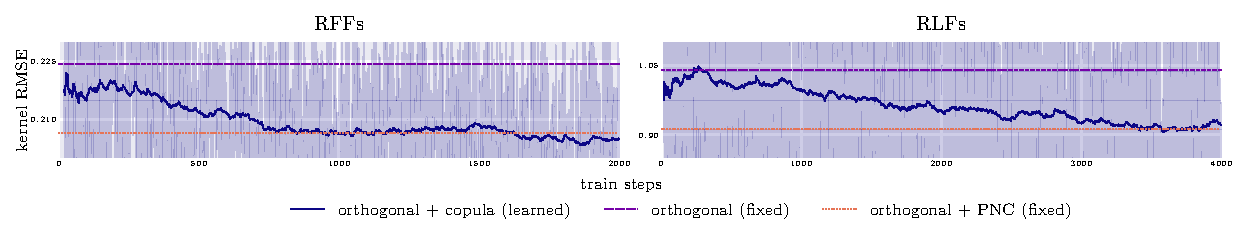
\includegraphics[width=\linewidth]{images/copula_training_curves.pdf}
    \caption{
        Training RMSE losses on a split of the Boston dataset.
        For the `orthogonal + copula (learned)' configuration, we display the raw training loss (light blue) as well as an exponential moving average (dark blue).
        The performance of the coupling scheme returned by optimising the copula matches the performance of the `orthogonal + PNC' scheme that we proved is optimal for the $m = 2$ case.
        The optimisation is very noisy but this can be mitigated by increasing the number of samples used in the reparameterisation trick.
    }
    \label{fig:boston-losses}
\end{figure}

\section{RFF and RLF experimental details} \label{app:rff_and_rlf_expts}
In this appendix, we supplement the discussion in Sec.~\ref{sec:rff_rlf_exps}, providing more details of our experimental setup for Gram matrix estimation.
We also apply norm-coupled RFs to sparse spectrum Gaussian processes \citep{lazaro2010sparse}, showing that in this case variance reduction does not help downstream performance.
We provide experimental details for the Performer \citep{choromanski2020rethinking} results in Table \ref{table:val_prec}.




\subsection{Details for RFF and RLF experiments} \label{app:rff_rlf_expt_details}

\pg{Overview}
In both our RFF and RLF experiments, we compare different coupling schemes for approximating the Gaussian kernel.
The Gaussian kernel, including a lengthscale parameter $\ell,$ an output scale variable $\sigma_v$ and a noise scale parameter $\sigma_n$, takes the form
$$k(x_i, x_j) = \sigma_v^2 \exp\left(-\frac{1}{2 \ell^2} ||\boldsymbol{x}_i - \boldsymbol{x}_j||_2^2\right).$$
Our baselines include standard methods for sampling random frequency vectors for use within RFFs and RLFs: i.i.d.~sampling and Halton sequences \citep{halton1960efficiency}.
In addition, for both settings, we consider ensembles of frequency vectors that are coupled to have orthogonal directions but i.i.d.~lengths.
For a dataset of dimension $d,$ for RFFs we use ensembles of $d$ orthogonal vectors.
For RLFs we use ensembles of $2d$ vectors, including $d$ orthogonal basis vectors and their $d$ antiparallel vectors.

\pg{Selecting kernel hyperparameters}
We want to compare our coupling schemes using realistic kernel hyperparameter values, which we determine as follows.
A realistic application setting for RFFs is within GPs for probabilistic regression.
Therefore, we first fit a GP on a tractable subset of the data, specifically a maximum of 256 randomly chosen datapoints, to select appropriate parameters  $\ell, \sigma_v$ and $\sigma_n.$
We optimise the exact GP marginal likelihood with respect to these hyperparameters, and subsequently fix them.
On the other hand, it is well-documented that RLFs suffer from poor estimator concentration when the data norm becomes large because of the exponential function in the feature map (Eq.~\ref{eq:rlf_exp}); see e.g.~Thm.~4 and App.~F6 of \citet{choromanski2020rethinking} or Thm.~4.3 of \citet{likhosherstov2022chefs}, where the authors bound the $L_2$-norm of queries and keys. 
This is anecdotally responsible for the deterioration in performance of Performers when networks become very deep. 
To reflect this fact and choose a data regime where vanilla RLFs can perform reasonably well (so we can assess any gains from our coupling), we set the lengthscale $\ell$ to two twice the average summed norm of the data, namely
\begin{equation}
    \ell = \frac{2}{N_\textrm{train}^2} \sum_{i,j=1}^{N_\textrm{train}} ||\boldsymbol{x}_i + \boldsymbol{x}_j||_2,
\end{equation}
over the training set.
We train the rest of the kernel parameters ($\sigma_v$ and $\sigma_n$) to maximise the marginal likelihood of the data under the exact GP.

%\pg{Optimising copula parameters}
%In order to learn the copula parameters $\boldsymbol{\theta},$ we optimise $\boldsymbol{\theta}$ on the training set (as described in App.~\ref{app:copulas}), and then evaluate the quality of the kernel approximation on a test set.

\pg{Splitting procedure}
To obtain mean evaluation metrics and standard errors, we evaluate the methods on multiple random splits as follows.
For each dataset, we conduct cross validation with 20 splits, splitting each dataset into a training and a test set.
Because we train an exact GP to determine kernel hyperparameters and evaluate its predictive NLL, we need to limit the number of datapoints used in both the training and the test set. 
We set them to a maximum of 256 points each by sub-sampling at random without replacement.
After training the GP, we evaluate the metrics on the test set, and repeat this procedure for all 20 splits.

\pg{Optimisation details}
We train the exact GP using the Adam optimiser \citep{kingma2014adam}, using a learning rate of $10^{-2}.$
The exact GP optimisation stage converges around $1000$ steps, and we run it up to $5000$ steps.
%The Gaussian copula optimisation stage is highly noisy, since the underlying Gaussian joint is resampled at each step.


\subsection{PNC RFFs for Gaussian processes} \label{app:are_predictions_improved?}
\pg{Kernel and posterior approximations}
%One natural question to ask is whether a better approximation to the kernel function leads to better downstream prediction, e.g.~GP regression.
Suppose that we have drawn an ensemble of frequency vectors from which we construct random features $\{\phi_{\text{RF}}(\boldsymbol{x}_i)_{i=1}^N\}$. 
Group these in a large design matrix $\boldsymbol{\Phi}$,
\begin{equation}
    \boldsymbol{\Phi} \coloneqq [\phi_{\text{RF}}(\boldsymbol{x}_i)]_{i=1}^N,
\end{equation}
where $\phi_{\text{RF}}(\boldsymbol{x}_i)$ of course depends on the ensemble frequencies $\{\boldsymbol{\omega}_i\}_{i=1}^m$ (suppressed for notational compactness).
For RFFs $\boldsymbol{\Phi} \in \mathbb{R}^{N \times 2m}$ whereas for RLFs $\boldsymbol{\Phi} \in \mathbb{R}^{N \times m}$.
We estimate the Gram matrix by $\widehat{\mathbf{K}} \coloneqq \boldsymbol{\Phi} \boldsymbol{\Phi}^\top$.

As noted by \citet{lazaro2010sparse}, this RF kernel approximation is exactly equivalent to a linear model, namely 
\begin{equation}
    \boldsymbol{y} = \boldsymbol{w} \boldsymbol{\Phi} + \boldsymbol{\epsilon},
\end{equation}
where $\boldsymbol{w} \sim \mathcal{N}(\boldsymbol{0}, \mathbf{I})$ and $\boldsymbol{\epsilon} \sim \mathcal{N}(\boldsymbol{0}, \sigma_n^2\mathbf{I}).$
The prior covariance of this linear model is $\boldsymbol{\Phi}^\top \boldsymbol{\Phi}  + \sigma_n^2 \mathbf{I},$ which is, by construction, equal in expectation to the exact covariance produced by the kernel, namely $\mathbf{K} + \sigma_n^2 \mathbf{I}$.
The predictive means of the approximate linear model and corresponding exact model are
\begin{align} \label{eq:mua1}
    \boldsymbol{\mu}_{\text{approx}} &= \boldsymbol{\Phi}_p\left(\frac{1}{\sigma_n^2}\boldsymbol{\Phi}_d \boldsymbol{\Phi}_d^\top + \boldsymbol{I}\right)^{-1}\boldsymbol{\Phi}_d\boldsymbol{y}, \\
    \boldsymbol{\mu}_{\text{exact}} &= \mathbf{K}_{pd} (\mathbf{K}_{dd} + \sigma_n^2 \mathbf{I})^{-1}\boldsymbol{y},
\end{align}
whereas the predictive covariances are
\begin{align} \label{eq:Ca1}
    \mathbf{C}_{\text{approx}} &= \boldsymbol{\Phi}_p^\top \left(\frac{1}{\sigma_n^2}\boldsymbol{\Phi}_d \boldsymbol{\Phi}_d^\top + \boldsymbol{I}\right)^{-1} \boldsymbol{\Phi}_p + \sigma_n^2 \mathbf{I}, \\
    \mathbf{C}_{\text{exact}} &= \mathbf{K}_{pp} - \mathbf{K}_{pd} (\mathbf{K}_{dd} + \sigma_n^2 \mathbf{I})^{-1}\mathbf{K}_{dp}.
\end{align}
Here, $\boldsymbol{\Phi}_d$ and $\boldsymbol{\Phi}_p$ are the design matrices corresponding to the training inputs and prediction outputs respectively, $\mathbf{K}_{dd}$ is the covariance matrix corresponding the training inputs, $\mathbf{K}_{pp}$ is the covariance matrix corresponding to the prediction inputs and $\mathbf{K}_{pd}$ and $\mathbf{K}_{dp}$ are the cross-covariance matrices between the training and prediction datapoints.
These models become exactly equivalent in the limit of an infinite number of features $m$ since the kernel approximation becomes exact.

We have seen that pairwise norm coupling improves the approximation of the Gram matrices $\mathbf{K}$. 
In particular, we are able to suppress the variance of each pointwise kernel estimate (Thm.~\ref{thm:pairwise_ot_solution} and Corr.~\ref{corr:norm_coupled_better}), and therefore the relative Frobenius norm error between the true and approximate Gram matrices (Table \ref{tab:rff}). 
In light of the discussion above, it would be natural to assume that this would result in more accurate approximations of the predictive mean and covariance.
However, in the following section we will see that surprisingly this is \emph{not} the case.

\pg{Evaluating posterior approximation quality}
Table \ref{tab:kld} takes the RFs from Sec.~\ref{sec:rff_rlf_exps}, where we found that our coupling can substantially improve the quality of kernel estimation. 
It then reports the KL divergence between the exact predictive posterior and the approximate predictive posteriors computed with RFFs and RLFs, respectively.
To be clear, Eqs \ref{eq:mua1} and \ref{eq:Ca1} can be rewritten
\begin{equation} \label{eq:approx_muandc}
    \boldsymbol{\mu}_{\text{approx}} = \widehat{\mathbf{K}}_{pd} (\widehat{\mathbf{K}}_{dd} + \sigma_n^2 \boldsymbol{I})^{-1}\boldsymbol{y},
    ~~~\mathbf{C}_{\text{approx}} = \widehat{\mathbf{K}}_{pp} - \widehat{\mathbf{K}}_{pd} (\widehat{\mathbf{K}}_{dd} + \sigma_n^2 \mathbf{I})^{-1}\widehat{\mathbf{K}}_{dp}
\end{equation}
where $\widehat{\mathbf{K}}_{dd} = {\mathbf{\Phi}}_d^\top {\mathbf{\Phi}}_d$, 
$\widehat{\mathbf{K}}_{pd} = {\mathbf{\Phi}}_d^\top {\mathbf{\Phi}}_p$,
$\widehat{\mathbf{K}}_{pd} = {\mathbf{\Phi}}_p^\top {\mathbf{\Phi}}_d$ and $\widehat{\mathbf{K}}_{pp} = {\boldsymbol{\Phi}}_p^\top {\boldsymbol{\Phi}}_p.$
It is then straightforward to compute the KL divergence between Gaussian distributions with means $ \boldsymbol{\mu}_{\text{approx}}$, $ \boldsymbol{\mu}_{\text{exact}}$ and covariances $\mathbf{C}_{\text{approx}}$, $\mathbf{C}_{\text{exact}}$.

\begin{table}[h!]
\resizebox{\textwidth}{!}{
\begin{tabular}{l c c c c c c}
\toprule
\scshape{Fourier Features} & \scshape{Concrete} & \scshape{Abalone} & \scshape{CPU} & \scshape{Power} & \scshape{Airfoil} & \scshape{Boston} \\
 \midrule
% \scshape{IID} & $1.487$ {\tiny $\pm 0.106$} & $0.038$ {\tiny $\pm 0.003$} & $1.860$ {\tiny $\pm 0.415$} & $0.151$ {\tiny $\pm 0.007$} & $0.358$ {\tiny $\pm 0.025$} & $2.123$ {\tiny $\pm 0.196$} \\
% \scshape{Halton} & $1.542$ {\tiny $\pm 0.104$} & $0.039$ {\tiny $\pm 0.003$} & $1.896$ {\tiny $\pm 0.417$} & $0.137$ {\tiny $\pm 0.006$} & $0.357$ {\tiny $\pm 0.024$} & $2.256$ {\tiny $\pm 0.203$} \\
% \scshape{Orthogonal} & $1.164$ {\tiny $\pm 0.113$} & $0.033$ {\tiny $\pm 0.004$} & $1.915$ {\tiny $\pm 0.424$} & $0.029$ {\tiny $\pm 0.002$} & $0.236$ {\tiny $\pm 0.017$} & $1.992$ {\tiny $\pm 0.191$} \\
% \scshape{+ PNC} & $1.163$ {\tiny $\pm 0.112$} & $0.032$ {\tiny $\pm 0.003$} & $1.870$ {\tiny $\pm 0.411$} & $0.029$ {\tiny $\pm 0.002$} & $0.235$ {\tiny $\pm 0.017$} & $1.988$ {\tiny $\pm 0.192$} \\
\scshape{i.i.d.} & $1.491$ {\tiny $\pm 0.106$} & $0.013$ {\tiny $\pm 0.001$} & $1.570$ {\tiny $\pm 0.417$} & $0.150$ {\tiny $\pm 0.007$} & $0.357$ {\tiny $\pm 0.025$} & $2.128$ {\tiny $\pm 0.197$} \\
\scshape{Halton} & $1.548$ {\tiny $\pm 0.104$} & $0.014$ {\tiny $\pm 0.001$} & $1.596$ {\tiny $\pm 0.419$} & $0.138$ {\tiny $\pm 0.006$} & $0.356$ {\tiny $\pm 0.024$} & $2.263$ {\tiny $\pm 0.204$} \\
\scshape{Orthogonal} & $1.166$ {\tiny $\pm 0.113$} & $0.004$ {\tiny $\pm 0.000$} & $1.635$ {\tiny $\pm 0.423$} & $0.029$ {\tiny $\pm 0.002$} & $0.235$ {\tiny $\pm 0.017$} & $1.990$ {\tiny $\pm 0.191$} \\
\scshape{+ PNC} & $1.168$ {\tiny $\pm 0.113$} & $0.004$ {\tiny $\pm 0.000$} & $1.589$ {\tiny $\pm 0.416$} & $0.029$ {\tiny $\pm 0.002$} & $0.235$ {\tiny $\pm 0.017$} & $1.985$ {\tiny $\pm 0.190$} \\
\midrule
\scshape{Laplace Features} & \scshape{Concrete} & \scshape{Abalone} & \scshape{CPU} & \scshape{Power} & \scshape{Airfoil} & \scshape{Boston} \\
 \midrule
% \scshape{IID} & $5.967$ {\tiny $\pm 0.363$} & $0.911$ {\tiny $\pm 0.102$} & $13.887$ {\tiny $\pm 8.971$} & $1.270$ {\tiny $\pm 0.083$} & $4.340$ {\tiny $\pm 0.472$} & $3.416$ {\tiny $\pm 0.378$} \\
% \scshape{Halton} & $6.264$ {\tiny $\pm 0.371$} & $0.864$ {\tiny $\pm 0.098$} & $13.733$ {\tiny $\pm 8.817$} & $0.978$ {\tiny $\pm 0.067$} & $4.004$ {\tiny $\pm 0.430$} & $4.013$ {\tiny $\pm 0.433$} \\
% \scshape{Orthogonal} & $4.706$ {\tiny $\pm 0.317$} & $0.588$ {\tiny $\pm 0.082$} & $12.808$ {\tiny $\pm 8.308$} & $0.434$ {\tiny $\pm 0.042$} & $3.083$ {\tiny $\pm 0.354$} & $2.759$ {\tiny $\pm 0.283$} \\
% \scshape{+ PNC + antithetic} & $4.781$ {\tiny $\pm 0.315$} & $0.587$ {\tiny $\pm 0.083$} & $12.919$ {\tiny $\pm 8.331$} & $0.512$ {\tiny $\pm 0.046$} & $3.086$ {\tiny $\pm 0.351$} & $2.769$ {\tiny $\pm 0.284$} \\
\scshape{i.i.d.} & $0.552$ {\tiny $\pm 0.064$} & $0.028$ {\tiny $\pm 0.003$} & $5.925$ {\tiny $\pm 1.961$} & $0.199$ {\tiny $\pm 0.011$} & $0.230$ {\tiny $\pm 0.024$} & $0.759$ {\tiny $\pm 0.068$} \\
\scshape{Halton} & $0.574$ {\tiny $\pm 0.064$} & $0.024$ {\tiny $\pm 0.003$} & $5.811$ {\tiny $\pm 1.897$} & $0.146$ {\tiny $\pm 0.009$} & $0.213$ {\tiny $\pm 0.022$} & $0.834$ {\tiny $\pm 0.074$} \\
\scshape{Orthogonal} & $0.486$ {\tiny $\pm 0.059$} & $0.014$ {\tiny $\pm 0.002$} & $5.494$ {\tiny $\pm 1.774$} & $0.059$ {\tiny $\pm 0.005$} & $0.165$ {\tiny $\pm 0.018$} & $0.679$ {\tiny $\pm 0.058$} \\
\scshape{+ PNC + antithetic} & $0.482$ {\tiny $\pm 0.058$} & $0.014$ {\tiny $\pm 0.002$} & $5.468$ {\tiny $\pm 1.780$} & $0.050$ {\tiny $\pm 0.006$} & $0.165$ {\tiny $\pm 0.018$} & $0.673$ {\tiny $\pm 0.058$} \\
\bottomrule
\end{tabular}
}
\vspace{1mm}
\caption{
    KL divergences (nats per datapoint) between exact and approximate GP predictive posterior on held out test sets.
    %Divergences are reported in nats.
    Note that we use $d$ features for RFFs and $2d$ features for RLFs.
    Reported errors are equal to two standard errors, i.e.~$98\%$ confidence intervals, computed by averaging across splits.
    Note that differences \emph{between} data splits are responsible for large errors; \emph{within} each split we take enough trials that the standard errors become small.
    For every individual data split, {\scshape{orthogonal}} is statistically significantly better than {\scshape{i.i.d.}} but there is no additional benefit from {\scshape{PW norm-coupled}}. 
    Results differ between splits because we consider a different subset of the dataset.
}
\label{tab:kld}
\end{table}

Surprisingly, we find that, even though our couplings improve the accuracy of kernel approximation, the approximate mean and covariance and hence the KL divergence to the true posterior do not necessarily improve. 
In Table \ref{tab:rff} we routinely see variance reductions of $10$-$20$\%, but even with very many trials this is not reflected in the data splits used for Table \ref{tab:kld}.

The reason for this experimental finding is that, as is clear in Eq.~\ref{eq:approx_muandc}, the posterior is highly nonlinear in \smash{$\widehat{\mathbf{K}}$}.
This is on account of the presence of matrix multiplications and inversions.
These nonlinear operations on the Gram matrix entries mean that, despite our \emph{pointwise} estimates being unbiased, $ \boldsymbol{\mu}_{\text{approx}}$ and $\mathbf{C}_{\text{approx}}$ are in fact biased. 
We have achieved our objective of variance reduction of \smash{$\widehat{\mathbf{K}}$} -- with pairwise norm coupling, it is both theoretically mandated and empirically observed.
But clearly this does not necessitate variance (or bias) reduction for $ \boldsymbol{\mu}_{\text{approx}}$ and $\mathbf{C}_{\text{approx}}$.
The relationship between the distribution of \smash{$\widehat{\mathbf{K}}$} and the distribution of the approximate posterior is more complex. 

\pg{Variance reduction does not always help predictive performance}
To sharpen this point, we now take a \emph{single} data split of the {\scshape{power}} dataset and plot the the kernel approximation RMSE (i.e.~kernel estimator variance), as well as various quantities of predictive interest, against the number of features $m$.
We exclude the Halton coupling (which is consistently worse than `orthogonal') for clarity of presentation.
Fig. \ref{fig:power_results} shows the results.

The left hand panel confirms that we have achieved our stated objective of variance reduction. 
Moreover, for all couplings the quality of approximation improves as we introduce more ensembles of size $d$.
Reading left to right, the other three panels show: (i) the KL divergence between the exact and approximate GP \emph{predictive posteriors} (as in Table \ref{tab:kld}), (ii) the predictive RMSE on a held out test set, and (iii) the KL divergence between the exact and approximate GP \emph{priors}.
In every instance, orthogonality provides a substantial gain but, despite the encouraging results for kernel RMSE, there is no additional benefit from PNC. 
However, it would be wrong to draw the simplistic conclusion that PNC does not give large enough variance savings to see downstream gains: comparable reductions from orthogonality yield substantial improvements. 
The problem is more fundamental, relating to how the joint distribution of kernel estimates -- beyond just the second moment of its pointwise entries -- interacts with nonlinear operations like matrix multiplication and inversion.
Table \ref{tab:pred-rmse} is a companion to Table \ref{tab:kld}, reporting predictive RMSEs as in Fig.~\ref{fig:power_results} for the other datasets.

\begin{table}[h!]
\resizebox{\textwidth}{!}{
\begin{tabular}{l c c c c c c}
\toprule
\scshape{Fourier Features} & \scshape{Concrete} & \scshape{Abalone} & \scshape{CPU} & \scshape{Power} & \scshape{Airfoil} & \scshape{Boston} \\
 \midrule
\scshape{i.i.d.} & $1.000$ {\tiny $\pm 0.027$} & $1.000$ {\tiny $\pm 0.043$} & $1.000$ {\tiny $\pm 0.179$} & $1.000$ {\tiny $\pm 0.016$} & $1.000$ {\tiny $\pm 0.025$} & $1.000$ {\tiny $\pm 0.067$} \\
\scshape{Halton} & $1.013$ {\tiny $\pm 0.027$} & $1.001$ {\tiny $\pm 0.043$} & $1.005$ {\tiny $\pm 0.179$} & $0.991$ {\tiny $\pm 0.016$} & $0.999$ {\tiny $\pm 0.025$} & $1.021$ {\tiny $\pm 0.068$} \\
\scshape{Sobol} & $1.010$ {\tiny $\pm 0.025$} & $1.000$ {\tiny $\pm 0.045$} & $1.004$ {\tiny $\pm 0.138$} & $0.991$ {\tiny $\pm 0.022$} & $0.997$ {\tiny $\pm 0.029$} & $1.027$ {\tiny $\pm 0.058$} \\
\scshape{Orthogonal} & $0.917$ {\tiny $\pm 0.026$} & $0.994$ {\tiny $\pm 0.044$} & $1.019$ {\tiny $\pm 0.182$} & $0.915$ {\tiny $\pm 0.019$} & $0.930$ {\tiny $\pm 0.025$} & $0.974$ {\tiny $\pm 0.066$} \\
%\scshape{+ PNC} & $0.918$ {\tiny $\pm 0.026$} & $0.994$ {\tiny $\pm 0.044$} & $1.011$ {\tiny $\pm 0.180$} & $0.915$ {\tiny $\pm 0.019$} & $0.929$ {\tiny $\pm 0.025$} & $0.974$ {\tiny $\pm 0.066$} \\
\scshape{+ PNC} & $0.917$ {\tiny $\pm 0.026$} & $0.994$ {\tiny $\pm 0.044$} & $1.033$ {\tiny $\pm 0.180$} & $0.915$ {\tiny $\pm 0.019$} & $0.930$ {\tiny $\pm 0.025$} & $0.975$ {\tiny $\pm 0.066$} \\
\midrule
\scshape{Laplace Features} & \scshape{Concrete} & \scshape{Abalone} & \scshape{CPU} & \scshape{Power} & \scshape{Airfoil} & \scshape{Boston} \\
 \midrule
\scshape{i.i.d.} & $1.000$ {\tiny $\pm 0.028$} & $1.000$ {\tiny $\pm 0.043$} & $1.000$ {\tiny $\pm 0.192$} & $1.000$ {\tiny $\pm 0.017$} & $1.000$ {\tiny $\pm 0.029$} & $1.000$ {\tiny $\pm 0.073$} \\
\scshape{Halton} & $1.007$ {\tiny $\pm 0.028$} & $0.997$ {\tiny $\pm 0.044$} & $1.003$ {\tiny $\pm 0.190$} & $0.964$ {\tiny $\pm 0.017$} & $0.989$ {\tiny $\pm 0.029$} & $1.019$ {\tiny $\pm 0.075$} \\
\scshape{Sobol} & $1.007$ {\tiny $\pm 0.025$} & $0.997$ {\tiny $\pm 0.045$} & $0.998$ {\tiny $\pm 0.176$} & $0.964$ {\tiny $\pm 0.022$} & $0.990$ {\tiny $\pm 0.039$} & $1.017$ {\tiny $\pm 0.071$} \\
\scshape{Orthogonal} & $0.979$ {\tiny $\pm 0.027$} & $0.990$ {\tiny $\pm 0.044$} & $1.003$ {\tiny $\pm 0.187$} & $0.899$ {\tiny $\pm 0.018$} & $0.958$ {\tiny $\pm 0.028$} & $0.979$ {\tiny $\pm 0.071$} \\
\scshape{+ PNC + antithetic} & $0.981$ {\tiny $\pm 0.027$} & $0.991$ {\tiny $\pm 0.044$} & $1.006$ {\tiny $\pm 0.187$} & $0.909$ {\tiny $\pm 0.018$} & $0.958$ {\tiny $\pm 0.028$} & $0.982$ {\tiny $\pm 0.071$} \\
%\scshape{Ortho. Corr} & $0.975$ {\tiny $\pm 0.027$} & $0.991$ {\tiny $\pm 0.044$} & $1.002$ {\tiny $\pm 0.187$} & $0.892$ {\tiny $\pm 0.018$} & $0.958$ {\tiny $\pm 0.028$} & $0.977$ {\tiny $\pm 0.071$} \\
\bottomrule
\end{tabular}
}
\vspace{2mm}
\caption{
    %Companion results to Table \ref{tab:kld} and Fig.~\ref{fig:power_results}, showing
    Predictive RMSEs (normalised to RMSE of {\scshape i.i.d.}) of the approximate GP predictive posteriors on held out test sets.
    Reported errors are equal to two standard errors, i.e.~$98\%$ confidence intervals, computed by averaging across splits.
   Substantially lower kernel estimator variance does \emph{not} guarantee better predictive performance, though performance tends to be no worse.}
\label{tab:pred-rmse}
\end{table}
\begin{figure}
    \centering
    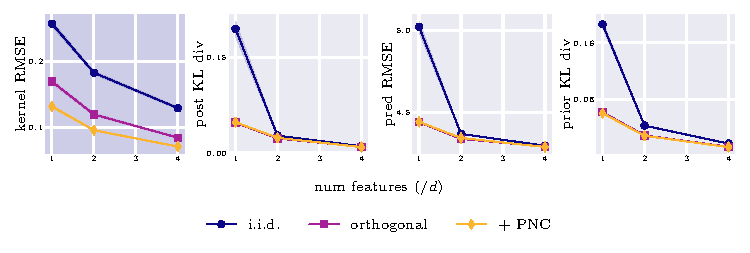
\includegraphics{images/power_results.pdf}
    \caption{Results on a single train-test split of the {\scshape{power}} dataset, showing kernel approximation RMSE, KL divergence to the true predictive posterior, test RMSE of predictions and KL divergence to the true prior.
    We have successfully reduced the variance of the kernel approximation, but this may not help downstream metrics.
    Standard errors are shaded but too small to easily see.}
    \label{fig:power_results}
\end{figure}

\subsection{Norm-coupled RLFs in Performers} \label{app:performers}
In Sec.~\ref{sec:rff_rlf_exps}, we used random Laplace features for attention approximation in Performers \citep{choromanski2020rethinking}, a type of efficient transformer that estimates softmax using a low rank decomposition.
Here, we discuss the results in greater detail.

\pg{Derivation of Eq.~\ref{eq:biased_attn_approx}}
Let $X_{ij}$ denote the random variable $\widehat{k}(\boldsymbol{x}_i, \boldsymbol{x}_j)$, which is an unbiased estimate of $\exp(\boldsymbol{x}_i^\top \boldsymbol{x}_j)$ constructed using features $\{\exp({\| \boldsymbol{x}_i \|^2}/{2}) \phi_\textrm{RLF}(\boldsymbol{x}_i) \}_{i=1}^N$.
Unbiasedness follows trivially from the fact that RLFs give an unbiased estimate of the Gaussian kernel.
Normalising by the sum of attention scores, let us define $\widehat{a}_{ij} \coloneqq X_{ij} / \sum_j  X_{ij}$.
Let $X_{ij} = \mu_{ij} + \delta_{ij}$ with $\mu_{ij} \coloneqq \mathbb{E}(X_{ij})$ and $\mathbb{E}(\delta_{ij})=0$.
Then
\begin{equation} 
\begin{multlined}
    \widehat{a}_{ij}^2 = (\mu_{ij}^2 + 2\mu_{ij}\delta_{ij} + \delta_{ij}^2)(\sum_k \mu_{ik} + \sum_k \delta_{ik})^{-2} 
    \\ = \frac{\mu_{ij}^2 + 2\mu_{ij}\delta_{ij} + \delta_{ij}^2}{N^2 \bar{\mu}_i^2} \left(1 - 2 \frac{\sum_k \delta_{ik}}{N \bar{\mu}_i} + 3 \frac{\sum_{kl} \delta_{ik}\delta_{il}}{N^2 \bar{\mu}_i^2}  + \mathcal{O}(\frac{1}{N^3}) \right),
\end{multlined}
\end{equation}
where we defined $\bar{\mu}_i \coloneqq \frac{1}{N}\sum_j \mu_{ij}$, the average groundtruth attention score across tokens. 
Since we are targeting $\frac{\mu_{ij}}{N \bar{\mu_i}}$,
\begin{equation} 
    \textrm{MSE}(\widehat{a}_{ij}) = \frac{1}{N^2 \bar{\mu_i}^2} \left(\delta_{ij}^2 - \frac{4 \mu_{ij} \delta_{ij}}{N \bar{\mu}_i} \sum_k \delta_{ik} + \frac{3\mu_{ij}^2}{N^2 \bar{\mu}_i^2} \sum_{kl} \delta_{ik} \delta_{il} \right) +  \mathcal{O}\left(\frac{1}{N^3}\right).
\end{equation}
As in the main text, denote $\textrm{MSE}(\widehat{a}_i)\coloneqq \frac{1}{N} \sum_j \textrm{MSE}(\widehat{a}_{ij})$, the average mean squared error over the tokens to which $i$ attends.
To better see the intuitive behaviour, suppose also that $\mu_{ij} = \bar{\mu}_i \hspace{0.2em} \forall \hspace{0.2em} j$. Then
\begin{equation} \label{eq:offset}
\begin{multlined}
    \textrm{MSE}(\widehat{a}_{i}) = \frac{1}{N^2 \bar{\mu_i}^2} \left(\frac{1}{N} \sum_j \delta_{ij}^2 - \frac{1}{N^2} \sum_{jk} \delta_{ij} \delta_{ik} \right) +  \mathcal{O}\left(\frac{1}{N^3}\right) 
    \\ =  \frac{1}{N^2 \bar{\mu}_i^2} \left( \frac{1}{N} \sum_{j} 
 \textrm{Var}(\widehat{k}(\boldsymbol{x}_i, \boldsymbol{x}_j)) - \frac{1}{N^2} \sum_{j, k}  \textrm{Cov}(\widehat{k}(\boldsymbol{x}_i, \boldsymbol{x}_{j}), \widehat{k}(\boldsymbol{x}_i, \boldsymbol{x}_{k})) \right) + \mathcal{O}\left(\frac{1}{N^3}\right),
    \end{multlined}
\end{equation}
as reported in Eq.~\ref{eq:biased_attn_approx}.

\pg{Positive monotone coupling}
In contrast to Eq.~\ref{eq:negative_monotone_coupling}, we say that random variables $(\omega_1,\omega_2)$ are \emph{postive monotone-coupled} if $\omega_1 = \omega_2$ almost surely.
This is a valid transport plan, the identity.
Clearly, all $m$ frequencies in an ensemble can be simultaneously positive monotone-coupled by making them equal.
It is intuitive that this should maximise the kernel estimator variance since we sample only one frequency lengthscale.
The proof is a trivial extension of the arguments made for Thm.~\ref{thm:pairwise_ot_solution} in App.~\ref{app:main_thm_rff_proof}, simply taking $c_\textrm{RLF} \to - c_\textrm{RLF}$ so that the support of the OT plan swaps.
We omit it for brevity.
It is also intuitive that this will increase the covariance between kernel estimates.

\pg{Variance, covariance, and attention approximation error}
Modifying the norm coupling between frequencies changes both \smash{$\textrm{Var}(\widehat{k}(\boldsymbol{x}_i, \boldsymbol{x}_j))$} and \smash{$\textrm{Cov}(\widehat{k}(\boldsymbol{x}_i, \boldsymbol{x}_{j}))$, so $\textrm{MSE}(\widehat{a}_{i})$} can change unpredictably. 
Fig.~\ref{fig:var_fig} shows the results for randomly $N=16$ synthetic, normally distributed $16$-dimensional keys, \smash{$\boldsymbol{x} \sim \mathcal{N}(0, \frac{1}{\sqrt{d}}\mathbf{I}_d$)}.
Strikingly, maximising the kernel estimator variance with a positive monotone (PM) coupling ends up \emph{improving} the quality of attention estimation since it also also increases the covariance between the unnormalised scores.
This counterintuitive finding shows highlights the limitations of variance reduction as a paradigm.

\begin{figure}
    \centering
    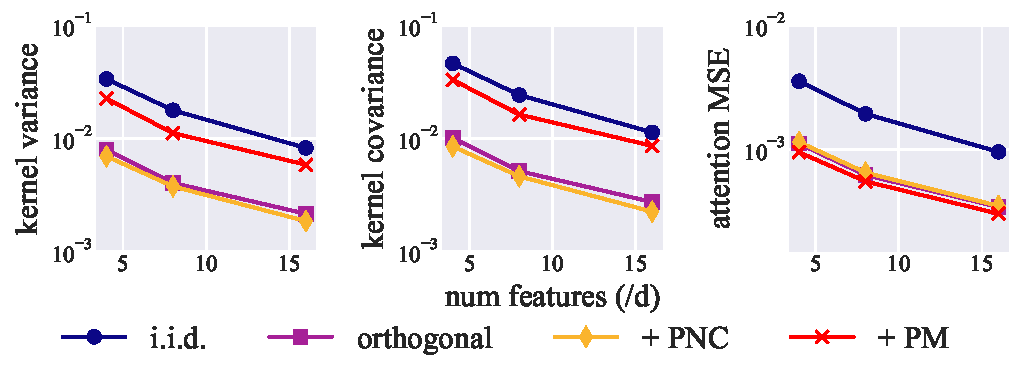
\includegraphics[width=0.65\linewidth]{images/attention_variance.pdf}
    \caption{Kernel variance $\textrm{Var}(\widehat{k}(\boldsymbol{x}_i, \boldsymbol{x}_j))$, kernel covariance $\textrm{Cov}(\widehat{k}(\boldsymbol{x}_i, \boldsymbol{x}_{j}))$ and attention mean squared error $\textrm{MSE}(a_i)$ plotted against number of frequencies for different coupling schemes. 
    As intended, PNC decreases the kernel estimator variance, 
    but it also decreases the kernel estimator covariance so the attention MSE remains essentially unchanged. 
    On the other hand, positive monotone coupling (PM) drastically increases both kernel variance (which it maximises) and kernel covariance. 
    The latter offsets the former (Eq.~\ref{eq:offset}), so that attention MSE actually drops: a remarkable, counterintuitive finding.}
    \label{fig:var_fig}
\end{figure}

\pg{Performer experimental details}
To obtain the results in Table \ref{table:val_prec}, we train a Performer-ViT \citep{dosovitskiy2020image, choromanski2020rethinking} on the ImageNet (1M) dataset \citep{deng2009imagenet}.
We estimate attention using $m=128$ random features that are orthogonal with norms that are: (i) i.i.d. (ii) PNC (Def.~\ref{def:coupled_norms_def}), or (iii) positive monotone-coupled (i.e. equal among blocks of size $d$).
We use a transformer with $12$ layers and heads, with hidden size $768$ and MLP dimension $3072$. 
We take $16 \times 16$ patches, and train with the Adam optimiser for $90$ epochs with a compound learning rate ($10^4$ steps linear warmup, constant, then cosine decay, with base LR $3 \times 10^{-3}$ and final LR $1 \times 10^{-5}$). 
The batch size is $4096$.
To get the standard errors, we average between $34$ and $48$ seeds per coupling.
We see that the lower attention MSE unlocked by PM coupling improves predictive performance over the baseline.


%A non-exhaustive list of publications with a substantial focus on reducing the variance of RF kernel estimates is given by: \citet{yu2016orthogonal, rowland2018geometrically, simrfs, likhosherstov2022chefs, qmc-rf, le2013fastfood, bojarski2017structured, choromanski2017unreasonable, lyu2017spherical, shen2017random, dao2017gaussian, munkhoeva2018quadrature}.
%This can sometimes be a very effective approach for improving downstream performance; e.g.~observe the benefits from $\sigma$-coupled GRFs in Sec.~\ref{sec:grfs}.
%But our findings suggest that the true reasons for any boost in performance are more complex than variance reduction alone. 
%There has been some recognition that other properties of the kernel approximation are important e.g.~for kernel ridge regression -- in particular, the spectral properties of \smash{$\widehat{\mathbf{K}}$} \citep{choromanski2018geometry,avron2017random} -- but we believe this to be underappreciated in the literature.
%More work is needed to fully identify the right desiderata for RF couplings in machine learning, and more algorithms to optimise couplings to improve them.
%OT provides an excellent framework for achieving this. 


%In our experiments, we have found that while pairwise coupling improves the accuracy of $\boldsymbol{\boldsymbol{K}}_{dd}, \boldsymbol{\boldsymbol{K}}_{pd}$ and $\boldsymbol{\boldsymbol{K}}_{pp},$ it did not improve the accuracy of $(\boldsymbol{\boldsymbol{K}}_{dd} + \sigma_n^2 \boldsymbol{I})^{-1},$ and therefore did not improve the overall accuracy of the approximate posterior.

\section{Graph random features} \label{app:grfs_all}
In this appendix, we provide a self-contained introduction to graph random features (GRFs) and previously proposed techniques to reduce their variance.
We also explain the motivations behind the series of approximations used in Sec.~\ref{sec:approximating_and_solving_grfs_ot}, and where possible provide empirical evidence that these approximations for tractability and efficiency do not substantially degrade the performance of the learned $\sigma$-coupling.

\subsection{Constructing graph random features} \label{app:grf_approx}
For the reader's convenience, we begin by providing a brief introduction to GRFs. 

\pg{Graph node kernels}
Recall that \emph{graph node kernels} $k: \mathcal{N} \times \mathcal{N} \to \mathbb{R}$ are positive definite, symmetric functions defined on pairs of nodes of $\mathcal{G}$. Note that one can also define kernels that take pairs of graphs as inputs, but these are not the object of our study. 

Many of the most popular graph node kernels in the literature are functions of weighted adjacency matrices \citep{smola2003kernels,chapelle2002cluster}. In particular, they are often functions of the \emph{graph Laplacian matrix},
\begin{equation}
    \mathbf{L} \coloneqq \mathbf{D} - \mathbf{W},
\end{equation}
where $\mathbf{W}$ is a (weighted) adjacency matrix and $\mathbf{D}$ is a diagonal degree matrix (satisfying $\mathbf{D}_{ii} = \sum_j \mathbf{W}_{ij}$). 
It is also common to consider its normalised variant,
\begin{equation} \label{eq:graph_lap}
    \widetilde{\mathbf{L}} \coloneqq \mathbf{D}^{-\frac{1}{2}} \mathbf{L} \mathbf{D}^{-\frac{1}{2}}, 
\end{equation}
whose spectrum is contained in $[0,2]$ \citep{chung1997spectral}. We provide examples in Table \ref{tab:taylor_expansions}.

\begin{table}[H]
\small
\centering
\begin{tabular}{cc}
\toprule
Name & Form  \\
\midrule
$d$-regularised Laplacian & $(\mathbf{I}_{N} + \sigma^2 \mathbf{L})^{-d}$   \\
$p$-step random walk & $(\alpha \mathbf{I}_{N} - \mathbf{L})^{p}, \alpha \geq 2$  \\
Diffusion   & $\exp(- \sigma^2 \mathbf{L}/2) $   \\
Inverse Cosine & $\cos \left(\mathbf{L} \pi /4 \right)$ \\
%Diffusion    & $\exp(\mathbf{W}-\sigma \mathbf{I}_{N}) $  & $...$  \\
\bottomrule
\end{tabular} \vspace{3mm}
\caption{Examples of graph node kernels. The $\mathrm{exp}$ and $\mathrm{cos}$ mappings are defined via Taylor series expansions rather than element-wise, e.g.~$\exp(\mathbf{M}) \coloneqq \lim_{n \to \infty} (\mathbf{I}_N + \mathbf{M}/n)^n$ and $\cos(\mathbf{M}) \coloneqq \textrm{Re}(\exp(i \mathbf{M}))$. $\sigma$ and $\alpha$ are regularisers.}\label{tab:taylor_expansions}
\normalsize
\end{table}

\textbf{Formula for graph random features.} Computing graph node kernels exactly is computationally expensive because of the $\mathcal{O}(N^3)$ cost of e.g.~matrix inversion or exponentiation. 
Inspired by the success of random Fourier features in the Euclidean domain \citep{rahimi2007random}, the recently-introduced class of \emph{graph random features} (GRFs) permits unbiased approximation of $k$ in subquadratic time \citep{graph_features,reid2023universal}.
Intuitively, GRFs interpret the powers of weighted adjacency matrices in the Taylor expansions of the expressions in Table \ref{tab:taylor_expansions} as weighted sums over walks on a graph. 
Instead of computing this infinite sum of walks exactly, we can sample $m$ finite walks (using importance sampling) to construct an unbiased estimate of $k$. 

Concretely, GRFs compute a set of estimators $\{\phi_\textrm{GRF}(v_i)\}_{i \in \mathcal{N}}$ such that $k(v_i,v_j) = \mathbb{E}[\phi_\textrm{GRF}(v_i)^\top \phi_\textrm{GRF}(v_j)]$ by taking:\footnote{Strictly, for unbiased estimation of diagonal kernel entries $\{k(v_i,v_i)\}_{v_i \in \mathcal{N}}$ we should construct \emph{two} independent sets of features, but this is found to make little practical difference \citep{reid2023universal} so we omit further discussion in this manuscript.}
\begin{equation}
    \phi_\textrm{GRF}(v_i) = \frac{1}{m} \sum_{k=1}^m \psi( \boldsymbol{\omega}_k^{(i)}),
\end{equation}
where $\boldsymbol{\omega}_k^{(i)}$ is the $k$th walk (out of a total of $m$) simulated out of the starting node $v_i$. We remind the reader that by a `walk' we mean a sequence of neighbouring graph nodes. 
The projection function $\psi(\cdot): \Omega \to \mathbb{R}^N$ maps from the set of graph random walks \smash{$\Omega \coloneqq \left \{(v_i)_{i=1}^l \,|\, v_i \in \mathcal{N}, (v_i,v_{i+1}) \in \mathcal{E}, l \in \mathbb{N} \right \}$} to a sparse $N$-dimensional feature vector.
It is computed as follows:
\begin{equation}
    \psi( \boldsymbol{\omega}^{(i)})_q \coloneqq \sum_{\omega_{iq} \in \Omega_{iq}} \frac{\widetilde{\omega}(\omega_{iq}) f(\textrm{len}(\omega_{iq}))}{p(\omega_{iq})} \mathbb{I}(\omega_{iq} \in \boldsymbol{\omega}^{(i)}), \quad q = 1,...,N.
\end{equation}
In this expression,
\begin{itemize}
    \item  $\psi( \boldsymbol{\omega}^{(i)})_q$ is the $q$th component of the feature projection of the random walk $\boldsymbol{\omega}^{(i)}$ (itself a sequence of neighbouring graph nodes beginning with $v_i$).
    \item $\Omega_{iq}$ is the set of \emph{all} graph walks between nodes $v_i$ and $v_q$, of which each $\omega_{iq}$ is a member. 
    \item $\mathbb{I}(\cdot)$ is the indicator function that evaluates to $1$ if its argument is true and $0$ otherwise. 
    \item $\omega_{iq} \in \boldsymbol{\omega}^{(i)}$ is the condition that $\omega_{iq}$, a particular walk between nodes $v_i$ and $v_q$, is a \emph{prefix subwalk} of $\boldsymbol{\omega}^{(i)}$, the random walk we actually sample.\footnote{Meaning that the walk $\boldsymbol{\omega}^{(i)}$ from node $v_i$ initially follows $\omega_{iq}$, then optionally continues to visit further nodes. Note the subtle difference in usage of the symbol $\in$ compared to in the expression $\omega_{iq} \in \Omega_{iq}$, where it means `a member of the set of walks' rather than `a prefix subwalk'.}
    \item $f: \mathbb{N} \to \mathbb{R}$ is the \emph{modulation function}, which controls the particular graph node kernel we choose to approximate. 
    \item $\textrm{len}(\omega_{iq})$ is the length of graph walk $\omega_{iq}$.
    \item $p(\omega_{iq})$ is the \emph{marginal probability} of sampling a random walk $\omega_{iq}$, which is known from the sampling strategy.
    \item $\widetilde{\omega}(\omega_{iq})$ is a function that returns the \emph{products of weights} of the edges traversed by $\omega_{iq}$.   
\end{itemize}
Intuitively, to construct $\psi(\boldsymbol{\omega}^{(i)})$ using a random walk $\boldsymbol{\omega}^{(i)}$, we look at the node that it visits at each of the \smash{$\textrm{len}(\boldsymbol{\omega}^{(i)})+1$} timesteps before termination. 
At every node, we add a contribution to the feature at the corresponding coordinate that depends on (i) the product of edge weights traversed so far, (ii) the known marginal probability of sampling the walk so far, and (iii) a `modulation function' $f$ applied to the number of steps taken so far.
We refer the reader to the original works of \citet{graph_features} and \citet{reid2023universal} for further technical details, experimental results and a proof of unbiasedness. 



\subsection{Antithetic termination} \label{app:antithetic_term}
In this section, we briefly describe \emph{antithetic termination} \citep{reid2023quasi}: a previously-proposed variance reduction algorithm that couples the lengths of pairs of random walks.  

Consider a random walker that terminates with probability $p$ at every timestep. 
In practice, this can be achieved by drawing a `termination random variable' $t$ from a uniform distribution on $[0,1]$, $t \sim \mathcal{U}([0,1])$, and ending the walk if $t<p$. 
Now consider two such walkers with corresponding termination random variables $t_1,t_2$. 
If they are independent, $t_1$ and $t_2$ are drawn independently. 
Antithetic termination instead proposes to induce a nontrivial joint distribution by first drawing $t_1 \sim \mathcal{U}([0,1])$ as usual, and then setting $t_2 = \mod_1(t_1 + \frac{1}{2})$. 
$t_2$ still follows a uniform marginal distribution so we preserve unbiasedness, but this coupling forces walkers to terminate at different timesteps (if $p_\textrm{halt}<0.5$) which the authors prove reduces the estimator variance under certain assumptions. 
This is one example of a possible hand-crafted coupling between random walk lengths that improves estimator concentration. 

It is also possible to improve the accuracy of estimators using graph random walks by coupling walker \emph{directions} \citep{reid2023repelling,luo2019distributed}. 
This approach is complementary to our own and can be combined with it. 
Formulating coupled walker directions in terms of OT is an interesting and involved technical challenge; we defer its study to future work. 

\subsection{Approximating the OT problem: details and discussion for Sec.~\ref{sec:approximating_and_solving_grfs_ot}} \label{app:what_are_the_approximations}

%\begin{figure}
%\centering \hspace{-8mm}
%    \includestandalone{grfs_master_schematic}
%\caption{The left schematic shows a permutation density $p_\sigma$ for the permutation $\sigma=$\lstinline{24351}, corresponding to a measure $\pi^{(\sigma)}$ on $[0,1]^2$.
%Both coordinates are pushed forward with \smash{$F_{\eta_\textrm{G}}^{-1}$} to get the coupling \smash{$\mu^{(\sigma)}$}.
%Then the permutation can be interpreted as a \emph{matching} between the quantiles of the geometric distribution over walk lengths, sketched in the central schematic.
%We use this to couple the lengths of pairs of walkers, shown on the right.
%Taking these walkers as inputs to the projection functions $\psi(\cdot)$ (Eq.~\ref{eq:projection_func}), we get $\sigma$-coupled GRFs.
%}\label{fig:permutation_walks_schematic} 
%\end{figure}

In this appendix, we discuss the steps to formulate the OT matching problem in Sec.~\ref{sec:approximating_and_solving_grfs_ot}. 
We will especially focus on the approximations needed to make the objective in Eq.~\ref{eq:ot_formulation} tractable, describing their motivation and where possible investigating how they modify the original objective. 
%For reference, Fig. \ref{fig:permutation_walks_schematic} gives an overview of the coupling mechanism.

To begin, we remind the reader of the OT formulation of the variance reduction problem for GRFs:
\small
\begin{equation} \begin{multlined} \label{eq:app_ot_formulation}
    \textrm{minimise }   \mathbb{E}_{(l_1^{(i)},l_2^{(i)}) \sim \mu, (l_1^{(j)},l_2^{(j)}) \sim \mu}  \left ( \mathbb{E}_\textrm{dirs} \left [ \left( \psi( \boldsymbol{\omega}_{1}^{(i)}) + \psi( \boldsymbol{\omega}_{2}^{(i)}) \right)^\top \left( \psi( \boldsymbol{\omega}_{1}^{(j)}) + \psi( \boldsymbol{\omega}_{2}^{(j)}) \right) \right]^2 \right)  
    \\ \textrm{for } \mu \in \Lambda_2(\eta_\textrm{G}),
\end{multlined}    
\end{equation}
\normalsize
where \smash{$\Lambda_2(\eta_\textrm{G})$} is the set of joint distributions on \smash{$\mathbb{N}^2$} with geometrically distributed marginals, \smash{$l_1^{(i)}$} is the length of walk \smash{$\boldsymbol{\omega}_1^{(i)}$} out of node $v_i$, $\mathbb{E}_\textrm{dirs}$ averages the \emph{directions} of walkers of a particular length, and \smash{$\psi( \boldsymbol{\omega}_k^{(i)})$} is the \emph{projection function} that maps from random walks to feature vectors (see Eq.~\ref{eq:projection_func}). 

\pg{Averaging walker trajectories}
As noted in the main text, the cost function in Eq.~\ref{eq:app_ot_formulation} is not analytically tractable. 
We can approximate it using MC sampling of graph random walks.
To do so, it will be convenient to introduce the \emph{direction-averaged feature vector} $\widetilde{\psi}(\cdot):\mathbb{N} \to \mathbb{R}^N$ satisfying
\begin{equation} \label{eq:dir_av_feat_proj}
    \widetilde{\psi}(l^{(i)}) \coloneqq \mathbb{E}_\textrm{dirs}[\psi( \boldsymbol{\omega}^{(i)})].
\end{equation} 
This computes the \emph{average} feature projection over all walks of a given length $l^{(i)}$ out of node $v_i$.
It is straightforward to estimate by simulating a finite number of random walks. 
If we move the expectation over walker directions \emph{inside} the square bracket, the (now approximate) OT problem becomes
\small
\begin{equation} \label{eq:app_approx_ot_formulation_1}
    \textrm{minimise } \mathbb{E}_{(l_1^{(i)},l_2^{(i)}) \sim \mu, (l_1^{(j)},l_2^{(j)}) \sim \mu}  \left [ \left( \widetilde{\psi}( l_{1}^{(i)}) + \widetilde{\psi}( l_{2}^{(i)}) \right)^\top \left( \widetilde{\psi}( l_{1}^{(j)}) + \widetilde{\psi}( l_{2}^{(j)}) \right) \right]^2 \textrm{ for } \mu \in \Lambda_2(\eta_\textrm{G}). 
\end{equation}
\normalsize
The price we pay is that we have ignored some higher-order corrections from the variance of the directions of the walks, but as we have seen in Sec.~\ref{sec:graph_gp_experiments} this does not prevent us from obtaining an effective, computationally cheap coupling.
%Note that we later again make this approximation to move the expectation over walk \emph{lengths} (now corresponding to a particular quantile of the geometric distribution) within the square brackets to arrive at Eq.~\ref{eq:approx_ot_formulation}.

\pg{Using $\sigma$-couplings} 
Unfortunately, Eq.~\ref{eq:app_approx_ot_formulation_1} remains intractable. 
To make progress, we must restrict our search-space of joint distributions from $\Lambda_2(\eta_\textrm{G})$ -- the set of \emph{all} joint distributions with geometrically-distributed marginals -- to a tractable subclass. 
Taking inspiration from approaches in numerical OT, we have considered the class of \emph{permutation densities} defined by $p_\sigma(x,y) \coloneqq n 1_{\sigma(\lceil nx \rceil) = \lceil ny \rceil}$,
 with $\sigma$ a permutation of order $n$ (that is, a bijection $\sigma: [\![n]\!] \to [\![n]\!]$), transformed coordinate-wise by pushing forward with the appropriate inverse CDF. 
This may initially seem an arbitrary choice, but it is motivated by three important observations. 
First, we have seen that this class of joint distributions frames the minimisation as a \emph{matching problem} which, under further simplifying assumptions, we can efficiently solve using techniques from linear programming.
Second, it is straightforward to sample from so the learned coupling will be practically useful. 
Third, it is well-motivated by results in discrete OT; see App.~\ref{app:discrete_ot_theory} for concrete theoretical guarantees. 
Once again, we have seen that in practice, even at modest permutation order $n$, this class contains couplings that can substantially outperform both i.i.d.~walkers and antithetic termination \citep{reid2023quasi}.

We now replace $\Lambda_2(\eta_\textrm{G})$ in Eq.~\ref{eq:app_approx_ot_formulation_1} by the set of measures $\{\mu^{(\sigma)} \}_{\sigma  \in S_n}$ obtained by pushing permutation densities through the required inverse CDF.
 $S_n$ is the set of permutations $[\![n]\!] \to [\![n]\!]$.
Denote by $\widehat{\psi}(\cdot) :[\![n]\!] \to \mathbb{R}^N$ the function
\begin{equation}
   \widehat{\psi}(q^{(i)}) \coloneqq \mathbb{E}_{u \sim \mathcal{U}((\frac{q-1}{n}, \frac{q}{n}])} \left( \widetilde{\psi}( F^{-1}_{\eta_\textrm{G}} (u)^{(i)})\right). 
\end{equation}
This takes the direction-averaged feature vector for node $v_i$ (see Eq.~\ref{eq:dir_av_feat_proj}) and evaluates a \emph{further} average over walk lengths corresponding to the $q$th quantile of the geometric distribution $\eta_\textrm{G}$.
Again, this is straightforward to estimate by simulating walks.
With a further approximation of the objective, we can consider 
\small
\begin{equation} \label{eq:approx_ot_formulation_matching}
    \sigma^* = \arg \min_{\sigma \in S_n}  \sum_{q_1 \in [\![n]\!]} \sum_{q_2 \in [\![n]\!]} \left [ \left( \widehat{\psi}( q_{1}^{(i)}) + \widehat{\psi}( \sigma(q_1)^{(i)}) \right)^\top \left( \widehat{\psi}( q_{2}^{(j)}) + \widehat{\psi}( \sigma(q_2)^{(j)}) \right) \right]^2 
\end{equation}
\normalsize
which is a matching problem.

\pg{Solving the matching problem}
Though we can now efficiently estimate the cost function with MC, it is is \emph{still} difficult to solve the matching problem in Eq.~\ref{eq:approx_ot_formulation_matching} efficiently because it is quadratic \citep{finke1987quadratic, burkard1998quadratic}.
Minimum weights quadratic bipartite matching problems are generally NP-hard, but here the problem has extra symmetry that makes it simpler.

In App.~\ref{sec:quad_grfs}, we discuss possible approaches to directly solve the matching problem in Eq.~\ref{eq:approx_ot_formulation_matching}. 
In particular, we prove that it can be solved with high probability at a time complexity independent of the number of nodes $N$, and give a polynomial time algorithm for the special case of diagonal kernel entries $k(v_i,v_i)$. 
Notwithstanding this progress, as a simpler first recourse we can just make a further approximation by restricting the sum to $q_1 = q_2$ diagonal terms.
This is the approximation used to get the results in the main text.
Doing so, we arrive at 
\small
\begin{equation} \label{eq:tractable_ot_formulation}
    \sigma^* = \arg \min_{\sigma \in S_n}  \sum_{q \in [\![n]\!]} \left [ \left( \widehat{\psi}( q^{(i)}) + \widehat{\psi}( \sigma(q)^{(i)}) \right)^\top \left( \widehat{\psi}( q^{(j)}) + \widehat{\psi}( \sigma(q)^{(j)}) \right) \right]^2. 
\end{equation}
\normalsize
This is now a minimum-weights bipartite matching problem with \emph{linear} weights. 
Even though the search space of possible permutations of order $n$ is of size $n!$, it is well known that it can be solved efficiently and exactly using algorithms from linear programming (e.g.~the Hungarian algorithm \citep{kuhn1955hungarian}) in time $\mathcal{O}(n^3)$. 
As stated in Sec.~\ref{sec:approximating_and_solving_grfs_ot} of the main text, we can use this optimal permutation to construct \emph{$\sigma$-coupled GRFs}.

This approximation might seem unreasonable since it involves discarding all the off-diagonal $q_1 \neq q_2$ terms from the objective, but for modest permutation order $n$ we can empirically test the effect this has on the quality of the obtained coupling.
We achieve this by comparing to the \emph{best} possible permutation obtained by exhaustively searching the $n!$ possibilities.

Fig. \ref{fig:approx_obj} plots the results for GRF estimates of the $2$-regularised Laplacian kernel on the \lstinline{eurosis} graph, comparing the approximate and exact objectives.
The former can be computed efficiently but the latter is evaluated at a cost exponential in $n$, so we limit to $n=10$ and smaller.
We plot the kernel approximation error (normalised by the i.i.d.~result) for different permutation orders.
We also plot the \emph{Cayley distance} between the permutations, which measures the difference between them.
As $n$ grows, the permutations become more different so we are clearly not finding the same coupling.
Nonetheless, we do not see a statistically significant difference in the amount of variance reduction.
This suggests that our linear proxy objective is reasonable.
We defer more detailed analytic study of this curious phenomenon to future work.


\begin{wrapfigure}{r}{0.61\textwidth}
\vspace{-6.6mm} \hspace{4mm}
    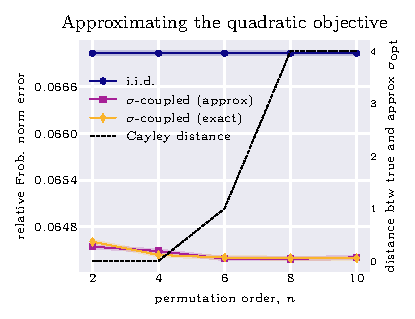
\includegraphics{images/approx_obj.pdf} 
     \vspace{-3mm}
\caption{Relative Frobenius norm error (normalised by i.i.d.~result) with permutations of order $n$ learned using exact and approximate objectives. 
`Cayley distance' shows the difference between the learned permutations. 
Although dropping off-diagonal terms from the objective in Eq.~\ref{eq:approx_ot_formulation_matching} changes the $\sigma$-coupling, it does not significantly detriment variance reduction. }\label{fig:approx_obj} \vspace{-3mm}
\end{wrapfigure} 
\textbf{How important are the approximations?}
This section has provided comprehensive details about the series of approximations required to make the GRF variance reduction OT problem tractable and solve it efficiently. 
We close by emphasising that, even if these approximations mean that we are not \emph{exactly} solving the original OT problem, we clearly nonetheless obtain a computationally efficient coupling that offers much greater variance reduction compared to heuristically-motivated techniques.
Analytic intractability is common in OT (Sec.~\ref{sec:rffs_and_rlfs} being an obvious exception), but fortunately this framework also equips us with a powerful arsenal of numerical tools to achieve our goal of finding effective, cheap sample couplings.
%We see that in action here, yielding principled couplings that outperform the previous state of the art.


\subsubsection{Proof of Thm.~\ref{thm:exact_soln}: towards an analytic solution to Eq.~\ref{eq:approx_ot_formulation_matching} }
\label{sec:quad_grfs}
To assuage any possible dissatisfaction with the $q_1=q_2$ approximation in Eq.~\ref{eq:tractable_ot_formulation}, in this section we discuss progress towards solving the optimisation problem in Eq.~\ref{eq:approx_ot_formulation_matching} \emph{exactly}.  %(Eq.~\ref{eq:ot_formulation} in the main body of the paper) 
In particular, we prove Thm.~\ref{thm:exact_soln}:
that it can be solved with high probability and
\begin{enumerate}
\item at a time complexity independent from the dimensionality of vectors  \smash{$\{\widehat{\psi}( q^{(i,j)})\}_{q=1}^n$} (at the cost of a one-time pre-processing), or
\item in polynomial time in the special case $i=j$ (under mild assumptions about the distribution of the averaged projection vectors \smash{$\{\widehat{\psi}( q^{(i,i)})\}_{q=1}^n$}).
\end{enumerate}

This is possible because of the extra structure in the quadratic matching problem.
A general efficient solution remains (for now) out of reach, but we hope this progress will spur further research in this direction.
Note especially that independence of the time complexity from the dimensionality of \smash{$\{\widehat{\psi}( q^{(i,i)})\}_{q=1}^n$} means that the difficulty of the optimisation does not depend on the number of nodes $N$: a very 
convenient property for large graphs.

\emph{Proof.} 
First, for clarity of exposition, we will introduce more convenient notation and important definitions. 
For a given $\epsilon>0$ and a vector $\mathbf{v} \in \mathbb{R}^{d}$, define the set $N_{\epsilon}(\mathbf{v})=\{\mathbf{w} \in \mathbb{R}^{d}:|\alpha_{\mathbf{v},\mathbf{w}}-\frac{\pi}{2}| \leq \epsilon\}$, where $\alpha_{\mathbf{v},\mathbf{w}}$ is an angle between $\mathbf{v}$ and $\mathbf{w}$.
Then define the property of \emph{$\epsilon$-separation} as follows.

\begin{definition} \label{def:eps_sep}
For a given $\epsilon>0$, a set of vectors $\mathcal{V}$ and a vector $\mathbf{v} \in \mathcal{V}$, we say that $\mathbf{v}$ is \emph{$\epsilon$-separated} in $\mathcal{V}$ if
\begin{equation}
N_{\epsilon}(\mathbf{v}) \cap \bigcup_{\mathbf{x} \in \mathcal{V} \backslash \{\mathbf{v}\}} N_{\epsilon}(\mathbf{x}) = \emptyset.
\end{equation}
\end{definition}

Simplifying notation, we can rewrite Eq.~\ref{eq:approx_ot_formulation_matching} as the following optimisation problem:
\begin{equation}
\label{eq:quad}
\sigma^* = \textrm{argmin}_{\sigma} \sum_{q_1, q_2 \in \{1,...,n\}}[(\mathbf{v}_{q_1}^{(i)}+\mathbf{v}_{\sigma(q_1)}^{(i)})^{\top}(\mathbf{v}_{q_2}^{(j)}+\mathbf{v}_{\sigma(q_2)}^{(j)})]^{2},    
\end{equation}
where $\sigma$ is the permutation of the sequence $(1,2,...,n)$
and $\mathbf{v}_{q}^{(i,j)} \coloneqq \widehat{\psi}( q^{(i,j)})$. 
With every permutation $\sigma$ of the sequence $(1,...,n)$, we will associate the perfect matching $M(\sigma)$ in its corresponding bipartite graph with monochromatic classes of size $n$ each. 
Denote 
\begin{equation}
\mathbf{f}^{(i)}_{M(\sigma)} \coloneqq \sum_{e \in M(\sigma)} \mathbf{u}_{e}^{(i)},    
\end{equation}
where $\mathbf{u}_{e}$ is given by 
\begin{equation}
\mathbf{u}_{(k,\sigma(k))}^{(i)}= \textrm{vec} \left [(\mathbf{v}_{k}^{(i)}+\mathbf{v}^{(i)}_{\sigma(k)}) \otimes (\mathbf{v}_{k}^{(i)}+\mathbf{v}_{\sigma(k)}^{(i)}) \right].   
\end{equation}
Here, $\otimes$ represents the outer product and $\textrm{vec}$ is the `vectorising' operation that flattens its input to a vector.
Note that that \smash{$\mathbf{u}_{(k,\sigma(k))} \in \mathbb{R}^{N^2}$}.

It is straightforward to see that, in this notation, the optimisation problem becomes
\begin{equation} \label{eq:rewritten_problem}
    \sigma^* = \textrm{argmin}_{\sigma}  {\mathbf{f}^{(i)}_{M(\sigma)}}^\top \mathbf{f}^{(j)}_{M(\sigma)}.
\end{equation}
We will now discuss progress towards solving this efficiently.

\pg{Making the problem independent of $N$}
Let us first show how we can make the optimisation problem independent of the number of nodes $N$ with high probability, at the cost of \vspace{0.25mm}a one-time pre-processing.
Our basic approach is to conduct \emph{dimensionality reduction} of the vectors \smash{$\mathbf{u}^{(i,j)}_e$} via the Johnson-Lindenstrauss Transform (JLT) \citep{jlt}.
Specifically, we compute
\begin{equation}
\widehat{\mathbf{u}}^{(i,j)}_{(k,\sigma(k))} = \frac{1}{\sqrt{r}}\mathbf{G}\mathbf{u}^{(i,j)}_{(k,\sigma(k))},  
\end{equation}
where $r \in \mathbb{N}$ denotes the number of random projections and 
$\mathbf{G} \in \mathbb{R}^{r \times N^{2}}$ is a Gaussian matrix with entries taken independently at random from $\mathcal{N}(0, 1)$.
From the well-known properties of JLT \citep{dasgupta_jlt}, we have that
\begin{equation}
\mathbb{E}[(\widehat{\mathbf{u}}^{(i)}_{(k,\sigma(k))})^{\top}\widehat{\mathbf{u}}^{(j)}_{(k,\sigma(k))}] = 
(\mathbf{u}^{(i)}_{(k,\sigma(k))})^{\top}\mathbf{u}^{(j)}_{(k,\sigma(k))} 
\end{equation}
since it is unbiased. 
We also have that
\begin{equation} \label{eq:jlt_conc}
    1-\epsilon \leq \frac{\|\widehat{\mathbf{u}}^{(i)}_{(k,\sigma(k))} \pm \widehat{\mathbf{u}}^{(j)}_{(k,\sigma(k))}\|^{2}_{2}}
{|\mathbf{u}^{(i)}_{(k,\sigma(k))} \pm \mathbf{u}^{(j)}_{(k,\sigma(k))}|^{2}_{2}} \leq 1+\epsilon,
\end{equation}
with $r=\mathcal{O}(\frac{\log(n)}{\epsilon^{2}})$ random projections, with probability $p  = 1 - \textrm{neg}(n)$.
Here, $\textrm{neg}$ denotes the negligible function of $n$.

Eq.~\ref{eq:jlt_conc} describes the ability of the JLT to (approximately) preserve $L_2$-norms.
The analogous property for preservation of dot-products also holds, which of interest to us given Eq.~\ref{eq:rewritten_problem}. 
It follows because for any $\mathbf{x},\mathbf{y}\in \mathbb{R}^{N^{2}}$,
\begin{equation}
\mathbf{x}^{\top}\mathbf{y} = \frac{\|\mathbf{x}+\mathbf{y}\|^{2}-\|\mathbf{x}-\mathbf{y}\|^{2}}{4}.
\end{equation}

The properties above lead us directly to an algorithm to decouple the time complexity of the optimisation from $N$.
One simply replaces every \smash{$\mathbf{u}^{(i,j)}_{(k,\sigma(k))}$} with its corresponding dimensionality-reduced \smash{$\widehat{\mathbf{u}}^{(i,j)}_{(k,\sigma(k))}$}
for \smash{$r=O(\frac{\log(n)}{\epsilon^{2}})$} and $\epsilon>0$ small enough. 
Then, by the concentration result listed above and the union bound over all pairs $(i, j)$, we conclude that the optimal 
$\sigma$ (potentially not unique) will remain optimal after applying the JLT (since all dot-products are approximately preserved). 
This completes the analysis.
We stress that $r$ does \emph{not} depend directly on the dimensionality of  \smash{$\mathbf{u}^{(i,j)}_{(k,\sigma(k))}$}, and therefore on $N$.

\pg{Polynomial in $n$ algorithm for $i=j$}
We can make further progress in the special case 
that $i=j$, i.e.~if we are minimising the variance of diagonal kernel entries $k(v_i,v_i)$. 
Denote by $T(n)$ time complexity of an efficient polynomial-time algorithm for solving the minimum weights matching problem on bipartite graphs with monochromatic parts of size $n$ each.
The following is true.

\begin{lemma} \label{lemma:k_matching_lemma}
If Eq.~\ref{eq:quad} has a unique solution $\sigma^{*}$ and furthermore $\mathbf{f}_{M(\sigma^{*})}$ is $\epsilon$-separated in $\mathcal{F}=\{\mathbf{f}_{M(\sigma)}: \sigma \in S_n\}$ for some $0<\epsilon<\frac{\pi}{2}$ (where $S_n$ denotes the set of all permutations of the sequence $(1,...,n)$), then, for any $k>0$, $\sigma^{*}$ can be found in time $k \cdot T(n)$ with probability $1-(1-p_{\epsilon})^{k}$.
Here, $p_{\epsilon}$ is given by the following formula:
\begin{equation}
p_{\epsilon} = 
\mathbb{P}\left[\left|\arccos \left(\frac{g_{1}}{\sqrt{g_{1}^{2}+...+g_{N^{2}}^{2}}} \right)-\frac{\pi}{2}\right| \leq \epsilon \right],    
\end{equation}
%\begin{equation}
%p_{\epsilon} = 
%\mathbb{P}\left[\left|\arccos(\widehat{\mathbf{g}}^\top \widehat{\mathbf{f}}_{M(\sigma^*)})-\frac{\pi}{2}\right| %\leq \epsilon \right]    
%\end{equation}
with $\mathbf{g} \in \mathbb{R}^{N^2}$ a random isotropic vector. 
\end{lemma}

\emph{Proof of Lemma \ref{lemma:k_matching_lemma}}.
If $i=j$, the expression in Eq.~\ref{eq:rewritten_problem} is simply $\|\mathbf{f}_{M(\sigma)}\|_{2}^{2}$.
%This uses the fact that the scalar product of dot-products can be rewritten as the dot-product of flattened outer-products. 
Thus, the goal is to find a permutation $\sigma$ that minimises the $L_2$-norm of the vector $\mathbf{f}_{M(\sigma)}$. 
%This leads to a particular instantiation of the quadratic matching problem.
We propose the following algorithm.
At every iteration, replace each vector $\mathbf{u}_{e}$ with the projection \smash{$u_{e} = \mathbf{u}_{e}^{\top}\mathbf{g}$} for $\mathbf{g} \in \mathcal{N}(0,\mathbf{I}_{N^2})$. %, where $r$ represents the dimensionality of vectors $\mathbf{u}$.
Note that, from $\epsilon$-separability, we have that if $\mathbf{g} \in N_{\epsilon}(\mathbf{v})$, then the permutation $\sigma$ corresponding to the minimum weight matching in the bipartite graph with weights given by $u_{e}$ is also equal to $\sigma^{*}$. 
This captures the intuition that the shortest vector will have the smallest projection on a random vector that is almost perpendicular to it, provided none of the other vectors are \emph{also} almost perpendicular to this projection direction.
From the fact that $\mathbf{g}$ is taken from the isotropic distribution, we know that the probability that $\mathbf{g} \in N_{\epsilon}(\mathbf{v})$ is exactly $p_{\epsilon}$, where $p_{\epsilon}$ is a geometrical constant that depends only on $N$.
Our algorithm solves the projected minimum weight matching problem (in time $T(n)$) at every iteration and stores the solution $\sigma$. 
Vectors $\mathbf{g}$ at different iterations are chosen independently. 
After $k$ iterations, the algorithm computes the original objective for every previously-obtained solution and selects the one with the smallest value. 
From the above, this returns the optimal permutation $\sigma^{*}$ with probability $1-(1-p_{\epsilon})^{k}$, which completes the proof. \qed

Having considered both claims, the proof of Thm.~\ref{thm:exact_soln} is complete. \qed


\section{Asymptotic optimality of permutation densities for variance reduction} \label{app:discrete_ot_theory}
In Sec.~\ref{sec:approximating_and_solving_grfs_ot} of the main text, we alluded to the choice of permutation densities $ p_\sigma(x,y) \coloneqq n 1_{\sigma(\lceil nx \rceil) = \lceil ny \rceil}$ depicted in Fig.~\ref{fig:main_grfs_schematic} being not only convenient (in terms of ease of sampling and optimising), but also well-motivated by results from OT theory. 
Here, we make this statement concrete, showing that in the limit of infinite permutation order $n$ this class contains the solution to a broad range of OT problems.

\begin{theorem}[Asymptotic optimality of permutation densities] \label{thm:optimality_app}
 Consider the class of joint measures $\Lambda^{(\sigma)} \coloneqq \{\mu^{(\sigma)}\}$ specified by permutations $\sigma$ of order $n$, given by permutation densities $p_\sigma$ pushed forward coordinate-wise using the (left-continuous) inverse CDF $F_\eta^{-1}$.
 Suppose also that the marginal measure $\eta$ is absolutely continuous with respect to Lebesgue measure. 
Consider also a \emph{continuous} function $f:\mathbb{R} \to \mathbb{R}$ whose expectation is to be estimated using $m=2$ coupled samples. 
In the limit $n\to \infty$, the class $\Lambda^{(\sigma)}$ contains measures that converge weakly to the optimal transport plan -- that is, the sample coupling which provides the smallest possible estimator variance.
\end{theorem}

\emph{Proof}. Consider the set $\{u_i \coloneqq \frac{1}{n} \left ( i - \frac{1}{2} \right) \}_{i=1}^n$ for some $n \in \mathbb{N}$. 
Consider also a random variable $X$ with measure $\eta \in \mathcal{P}(\mathbb{R})$ and corresponding distribution function $F$. 
Define its left-continuous inverse $F^{-1}(y) \coloneqq \inf \{x \in \mathbb{R}: F(x) \geq y \}$.
Given some permutation order $n \in \mathbb{N}$, consider the set  
\begin{equation}
    \left \{ x_i \coloneqq F^{-1}\left(u_i\right) = F^{-1}\left(\frac{i-\frac{1}{2}}{n}\right)  \right \}_{i=1}^n 
\end{equation}
which we will refer to as the \emph{quantile midpoints}. Then consider the discrete measure
\begin{equation}
\eta_n \coloneqq \frac{1}{n} \sum_{i=1}^n \delta_{x_i}
\end{equation}
where $\delta_{x_i}(A)=1$ if $x_i \in A$ and $0$ otherwise (with $A \subset \mathbb{R}$). 
Denote by $F_n$ the distribution associated with $\eta_n$.
Clearly, $\eta_n \to \eta$ weakly as $n \to \infty$ since $F_n(x) \to F(x)$ for any continuity point $x$ of $F$ \citep{billingsley2013convergence}. 
In this sense, the measure $\eta_n$ is a discrete approximation to $\eta$. 

Now consider the variance reduction OT problem for estimating $\mathbb{E}_{\omega \sim \eta}[f(\omega)]$ with $m=2$ samples,
\begin{equation} \label{eq:ot_formulation_asymptotic}
    \mu^* = \textrm{arg min}_{\mu \in \Lambda_2(\eta)} \left [ \mathbb{E}_{(\omega_1, \omega_2) \sim \mu}  f(\omega_1)f(\omega_2) \right].
\end{equation}
Solving this analytically for arbitrary $f$ is not in general tractable. 
On the other hand, if we instead take the discretised marginals $\eta_n$, we must solve
\begin{equation} \label{eq:ot_formulation_asymptotic_discrete}
    \mu_n^* = \textrm{arg min}_{\mu \in \Lambda_2(\eta_n)} \left [ \mathbb{E}_{(\omega_1, \omega_2) \sim \mu}  f(\omega_1)f(\omega_2) \right].
\end{equation}
This special case of discrete marginal measures where all points have equal mass can be solved \emph{exactly}. 
Our discussion is based on the proof outlined in the introduction to \citet{villani2021topics}, to which the interested reader is directed for full details.

\pg{OT with equal-mass discrete marginal measures} 
Any measure in $\Lambda_2(\eta_n)$ can be represented as a bistochastic $n \times n$ matrix $\mathbf{B} = [B_{ij}]_{i,j=1}^N \in \mathcal{B}_n$, meaning that all $B_{ij}$ are nonnegative and satisfy
\begin{equation}
    \sum_i B_{ij} = 1 \; \forall \; j;   \quad \sum_j B_{ij} = 1 \; \forall \; i.
\end{equation}
Therefore, the Kantorovich problem reduces to
\begin{equation}
    \inf_{B \in \mathcal{B}_n} \left [ \frac{1}{n} \sum_{ij} B_{ij} C_{ij} \right ]
\end{equation}
where we have encoded the transport costs in the cost matrix $\mathbf{C}= [f(x_i)f(x_j)]_{i,j=1}^n$.  
$B_{ij}$ is interpreted as the mass of the singleton $(x_i,x_j)$. 
This is a linear minimisation problem on a convex bounded set. 
It is well known that a solution always exists and corresponds to the convex hull of optimal permutation matrices. 
In more detail: by Choquet's theorem the problem admits solutions which are at the extremal points of $\mathcal{B}_n$ (points that cannot be written as a nontrivial linear combination of other points in $\mathcal{B}_n$). 
By Birkhoff's theorem these are exactly the permutation matrices $\mathbf{B}^{(\sigma)} \coloneqq [\delta_{\sigma(i)j}]_{i,j=1}^n$ with $\sigma \in S_n$. 
So the optimal discrete coupling is the convex hull of the discrete joint measures corresponding to the set of optimal permutations.
See the work of \citet{villani2021topics} for further details.
Choosing just one of these optimal permutations $\sigma$ (since any convex combination of the corresponding measures will give the same amount of variance reduction), we have that
\begin{equation}
    \mu_n^* = \mu_n^{(\sigma)} \coloneqq \sum_{i=1}^n \frac{1}{n} \delta_{(x_i, x_{\sigma(i)})}. 
\end{equation}

%Mapping each $x_i$ back to its corresponding $u_i$\footnote{Note that this mapping may not be unique for discrete marginals $\eta$ with to discontinuous distributions $F_\eta$, but for our purposes it is sufficient to consider the bijection $x_i \to u_i$ since this will always give a measure $\smash{\mu^{(\sigma)}_n}$ that is equal to $\smash{\pi^{(\sigma)}_n}$ when transformed using the well-defined left-continuous inverse $F_\eta^{-1}(\cdot)$. The (lack of) uniqueness of $\smash{\mu^{(\sigma)}}$ is a detail that does not matter for sampling purposes.}, we obtain the joint distribution on $[0,1]^2$
%\begin{equation}
%    \mu_n^{(\sigma)} \coloneqq \sum_{i=1}^n \frac{1}{n} \delta_{(u_i, u_{\sigma(i)})}. 
%\end{equation}
%These correspond to the solutions of Monge's problem which are matchings between the source and target points $\{x_i\}$ (or $\{u_i\}$). Since we care about obtaining a coupling that minimises the estimator MSE it will be sufficient to consider just one of the optimal permutations among the set (whose cardinality will depend on the problem's symmetry). This measure looks very much like the canonical permutons depicted in Fig. \ref{fig:permuton_schematic}, but in lieu of `tiles' we have delta masses at the quadrant midpoints. 

\pg{Stability of OT plans} Another important result in optimal transport is the \emph{stability of transference plans}: namely, that if $\eta_n \to \eta$ weakly then the optimal coupling $\pi_n \in \Lambda_2(\eta_n)$ also converges to the optimal $\pi \in \Lambda_2(\eta)$ weakly provided the cost function $c(X_i,X_j)$ (in our case $f(X_i)f(X_j)$) is continuous and 
\begin{equation}
    \limsup_{n \to \infty} \int c(x_1,x_2) \textrm{d}\pi_n(x,y) < \infty.
\end{equation}
This important observation underpins the effectiveness of numerical approximations to optimal transport. We direct the reader to Thm.~1.7.2 by \citet{panaretos2020invitation} for a proof sketch and Thm.~5.20 by \citet{villani2009optimal} for more detailed exposition. It follows that $\mu_n^{*}$ converges weakly to the true optimal coupling $\mu^*$.

\pg{The OT plan is (asymptotically) in our search class}
Lastly, we have that our search class of couplings $\Lambda^{(\sigma)}$ (corresponding to permutation densities pushed forward by $F_\eta^{-1}$) contains measures that converge in distribution to \smash{$\mu_n^{(\sigma)}$} when $n \to \infty$. 
In this mathematical sense, the asymptotic limit the class of couplings amongst which we optimise includes measures that give the greatest possible variance reduction: roughly speaking, our method is `asymptotically optimal'.
This is intuitive because as the order of the permutation grows each `tile' of nonzero density narrows and can be increasingly well-approximated by a delta function. 


To see this, consider the measure on $[0,1]^2$ described by the permutation density $p_\sigma(x,y) = n 1_{\sigma(\lceil nx \rceil) = \lceil ny \rceil}$.
Consider also the discrete measure on $[0,1]^2$ given by
$\frac{1}{n} \sum_{i=1}^n \delta_{u_i}$ with the set $\{u_i\}_{i=1}^n$ the quantile midpoints defined previously. 
These measures converge in distribution (their corresponding joint CDFs can differ by at most $\frac{1}{n}$ at any point, which goes to $0$ as $n\to\infty$).
They will also converge in distribution when pushed forward coordinate-wise by $F_\eta^{-1}$ by continuity of $\eta$.
It follows that at asymptotic $n$ \smash{$\mu_n^{(\sigma)}$} and \smash{$\mu^{(\sigma)}$} converge in distribution, which completes the proof. \qed

We remark that not all the assumptions in Thm.~\ref{thm:optimality_app} hold in the GRF setting.
In particular, neither the marginal measure $\eta$ nor the function $f$ is continuous. 
The intention of including Thm.~\ref{thm:optimality_app} is to build intuition for the reader and provide some motivation for our choice of permutation densities.
We defer a rigorous investigation into relaxing these restrictive assumptions -- a tough measure-theoretic problem -- to future work. 

\section{Estimating PageRank}\label{app:pagerank}
In this appendix, we demonstrate a further use of the variance reduction OT techniques developed for graph random walks in Sec.~\ref{sec:grfs}: estimating the \emph{PageRank} vector \citep{page1998pagerank}.
This popular measure of the relative importance of the nodes $\mathcal{N}$ of a graph is expensive to compute exactly so is often estimated by sampling random walks \citep{fogaras2005towards}.
We will show that OT can be used to find a coupling between the walks to reduce the estimator variance, demonstrating the versatility of our approach beyond improving RFs. 

\subsection{Setup: estimating PageRank with random walks} \label{app:pr_bg}
The PageRank vector is the stationary distribution of  Markov chain whose state space is the set of all graph nodes $\mathcal{N}$, with a transition matrix
\begin{equation} \label{eq:def_p_tilde}
    \widetilde{\mathbf{P}} \coloneqq (1-p_\textrm{halt})\mathbf{P} + \frac{p_\textrm{halt}}{N} \mathbf{E}.
\end{equation}
Here, $p_\textrm{halt} \in (0,1)$ is a scalar, $N$ is the number of nodes and $\mathbf{E}=[1]_{i,j \in \mathcal{N}}$ is a matrix whose entries are all ones. $\mathbf{P}$ is the transiton matrix of a simple random walk,
\begin{equation} \label{eq:srw_transition}
    P_{ij} = \begin{cases}
        \frac{1}{d_i} & $if $ (i,j) \in \mathcal{E} \\
        0 & $otherwise$
    \end{cases}
\end{equation}
with $d_i$ the degree of the $i$th node. Since $\smash{\widetilde{\mathbf{P}}}$ is stochastic, aperiodic and irreducible, we define the unique PageRank vector $\boldsymbol{\rho} \in \mathbb{R}^N$:
\begin{equation}
    \boldsymbol{\rho}^\top \widetilde{\mathbf{P}} = \boldsymbol{\rho}^\top, \hspace{3mm} \boldsymbol{\rho}^\top \boldsymbol{1} = 1,
\end{equation}
where we normalised the sum of vector entries to $1$. Computing $\boldsymbol{\rho}$ analytically is expensive. Rearranging and Taylor expanding $(1 - (1-p_\textrm{halt})\mathbf{P})^{-1}$, it is straightforward to see that
\begin{equation}
    \boldsymbol{\rho}_i = \frac{p_\textrm{halt}}{N} \sum_{j \in \mathcal{N}} \sum_{k=0}^\infty (1-p_\textrm{halt})^k \mathbf{P}^k_{ji}.
\end{equation}
This is simply a sum over all walks from each of the graph nodes $v_j$ to node $v_i$, weighted by their respective probabilities -- that is, the expected number of random walkers ending at node $v_i$ if they terminate with probability $p_\textrm{halt}$ at every timestep -- which invites the estimator proposed by \citet{fogaras2005towards},
\begin{equation}
    \widehat{\boldsymbol{\rho}}_i = \frac{1}{Nm} \sum_{v_j \in \mathcal{N}} \sum_{n=1}^m \mathbb{I} [ n\textrm{th walk from node } v_j\textrm{ terminates at node} \hspace{1mm} v_i]. 
\end{equation}
An interesting and practically important question is whether the variance of the estimator $\widehat{\boldsymbol{\rho}}$ can be improved by coupling random walks.
As with GRFs, this can be achieved using antithetic termination \citep{reid2023quasi} (see Sec.~\ref{app:antithetic_term}).
However, we will see that our OT length coupling approach does equally well or better.

\subsection{OT formulation of PageRank variance reduction}
 Given $m=2$ walks, the variance of the PageRank estimator $\textrm{Var}(\widehat{\boldsymbol{\rho}}_i)$  depends on the quantity
 \small
 \begin{equation}
 \begin{multlined}
     \mathbb{E}(\widehat{\boldsymbol{\rho}}_i^2) = \mathbb{E} \bigg[ \frac{1}{N^2m^2} \sum_{v_j, v_k \in \mathcal{N}} \sum_{n_1, n_2=1}^2 \mathbb{I} [ n_1\textrm{th walk from node } v_j\textrm{ terminates at node} \hspace{1mm} v_i] \bigg.
     \\ \bigg.  \cdot  \mathbb{I} [ n_2\textrm{th walk from node } v_k\textrm{ terminates at node} \hspace{1mm} v_i] \bigg].
 \end{multlined}
 \end{equation}
 \normalsize
 After a few lines of algebra, the OT problem to minimise this quantity is 

\small
 \begin{equation} 
 \begin{multlined}
    \textrm{minimise } \mathbb{E}_{(l_1,l_2) \sim \mu} \sum_{v_j \in \mathcal{N}} \mathbb{P}[\textrm{RW of length $l_1$ from node $v_j$ terminates at node $v_i$}]
    \\ \cdot \mathbb{P}[\textrm{RW of length $l_2$ from node $v_j$ terminates at node $v_i$}] \textrm{ for } {\mu \in \Lambda_2(\eta_\textrm{G})}
\end{multlined}
\end{equation}
\normalsize
without making any approximations. 
$\mathbb{P}(\cdot)$ denotes the probability of the event in brackets.
As with GRFs, for tractability we restrict our search space of joint distributions to permutation densities pushed forward coordinate-wise with the geometric distribution inverse CDF, and this becomes
\small
\begin{equation} \label{eq:matching_pagerank}
\begin{multlined}
    \sigma^* = \arg \min_{\sigma} \sum_{v_j \in \mathcal{N}} \sum_{q \in [\![n]\!]} \mathbb{P}[\textrm{RW with length in $q$th quadrant from node $v_j$ terminates at node $v_i$}]
    \\ \cdot \mathbb{P}[\textrm{RW with length in $\sigma(q)$th quadrant from node $v_j$ terminates at node $v_i$}]. 
\end{multlined}
\end{equation}
\normalsize
The probabilities can be efficiently estimated by simulating random walks on the graph and recording where they terminate. 
This leaves us with a minimum-weights bipartite matching problem which can as usual be solved efficiently with the Hungarian algorithm \citep{kuhn1955hungarian}.

Note that we made fewer simplifications than for GRFs (Sec.~\ref{app:grf_approx}). 
They only requirements for tractability are restricting the class of considered joints to $\sigma$-couplings and computing MC estimates of the terms in the OT cost matrix.
We do not need to e.g.~move $\mathbb{E}_\textrm{dirs}$ inside a square or approximate a quadratic matching problem by a linear-weights counterpart. 


\subsection{Empirical results for PageRank} \label{app:more_pagerank_results}
\begin{figure}
    \centering
    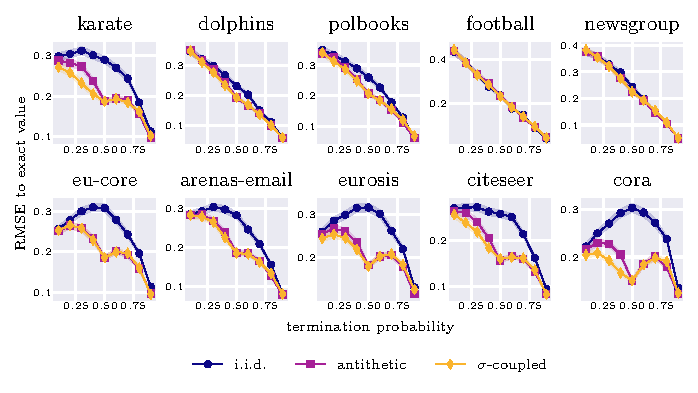
\includegraphics{images/pagerank_more_graphs_14_may.pdf}
    \caption{PageRank estimator errors $\|\boldsymbol{\rho} - \widehat{\boldsymbol{\rho}}\|_2$ for a range of real-world graphs when $2$ random walkers are taken to be i) i.i.d., ii) antithetic or iii) $\sigma$-coupled. Lower is better. The error is always at least as small and often substantially better when the walkers are coupled using our OT coupling. 
    One standard error is shaded.}
    \label{fig:pagerank_results}
\end{figure}
We now provide experiments using our OT coupling to improve the convergence of PageRank estimates. 
Fig. \ref{fig:pagerank_results} shows the results.
For termination probabilities $p_\textrm{halt} \in \{0.1,0.2,0.3,0.4,0.5,0.6,0.7,0.8,0.9 \}$, we compute the optimal permutation $\sigma$ by solving the matching problem in Eq.~\ref{eq:matching_pagerank} on an Erd\H os-R\`enyi graph with $N=100$ nodes, taking permutation order $n=10$ as a hyperparameter.
We then test these couplings on a range of real-world graphs \citep{community_graphs} of different sizes, plotting the estimator error $\|\boldsymbol{\rho} - \widehat{\boldsymbol{\rho}}\|_2$ (where $\boldsymbol{\rho}$ is the true PageRank vector and $\widehat{\boldsymbol{\rho}}$ is its MC estimate) against the termination probability $p_\textrm{halt}$. 
We include walkers that are i.i.d., antithetic \citep{reid2023quasi} and $\sigma$-coupled. 
At every value of $p_\textrm{halt}$, our method performs \emph{at least as well} as the baselines, and in some cases (e.g.~on the very large \lstinline{cora} graph) it gives much greater variance reduction.

Note that we only consider connected subgraphs and take $1000$ repeats for standard errors. 
Reading the plots from left to right for the top row and then the bottom, the number of nodes are: $\{ 34,62,105,115,398,986,1133,1272,2120,2708\}$. 
The shape of the curve and size of the gain from coupling depends on the particular graph being considered. 
For some graphs it is not possible to obtain a big reduction in PageRank estimator variance by coupling walkers (e.g.~\lstinline{football} and \lstinline{newsgroup}), so neither antithetic termination nor our $\sigma$-coupling can provide a big gain. 
A detailed investigation of how these observations relate to the mathematical graph structure is deferred to future work. 

\section{GRFs for GPs: additional details and experimental results} \label{app:grfs_for_gps}
In this appendix, we supplement Sec.~\ref{sec:graph_gp_experiments} by providing further experimental results for GRFs, including Gram matrix estimation on a wider range of graphs and a scalable graph-based GP on a different real-world dataset.
We also provide technical background and tedious details considered too long for inclusion in the main text.

\subsection{More results for Gram matrix estimation} \label{app:more_grf_results}
First, we run the experiment in the first part of Sec.~\ref{sec:graph_gp_experiments} for more real-world graphs.
 We approximate the $2$-regularised Laplacian kernel $\smash{(\mathbf{I} - \sigma^2 \widetilde{\mathbf{L}})^{-2}}$ with a regularisation parameter $\sigma=1$ and $m=2$ walkers. 
 Fig. \ref{fig:grfs_more_graphs} shows the results, with the kernel approximation error normalised by the i.i.d.~result (unlike in Fig. \ref{fig:permuton_grf}) for clarity of comparison.
 The $\sigma$-coupling consistently reduces the estimator variance, providing equally good or better results compared to the hand-crafted antithetic termination algorithm.
 The size of the gain depends on the graph structure. %, but $\sigma$-coupled walkers are always at least as good as both the i.i.d.~and antithetic termination baselines. 
 %More work is needed to characterise the type of graph for which coupling walk lengths gives the biggest reductions in kernel estimator error.

\begin{figure} 
    \centering
    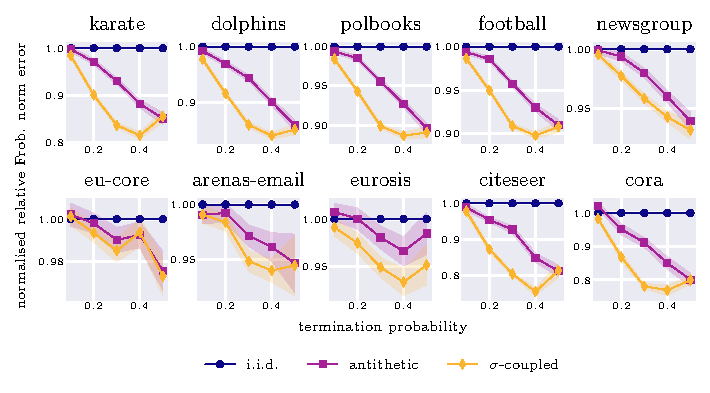
\includegraphics{images/grfs_more_graphs_14th_may.pdf}
    \caption{Relative Frobenius norm error $\|\mathbf{K} - \widehat{\mathbf{K}}\|_\textrm{F} / \| \mathbf{K} \|_\textrm{F}$ between true and approximated Gram matrices for different termination probabilities when walkers are i) i.i.d., ii) antithetic \citep{reid2023quasi} or iii) $\sigma$-coupled using our OT approach. 
    All results are normalised by the i.i.d.~variance for easy comparison. 
    Lower is better. 
    The $\sigma$-coupling is consistently as good or better across values of $p_\textrm{halt}$ and graph topologies and sizes.
    One standard error is shaded. \vspace{-5mm}}
    \label{fig:grfs_more_graphs}
\end{figure}

\subsection{Scalable GPs on graphs}
\pg{A very short introduction to graph-based GPs}
%Gaussian process (GP) models have become an indispensible workhorse of probabilistic machine learning, providing a framework for learning unknown functions in a manner that incorporates prior information and provides well-calibrated uncertainty estimates \citep{williams2006gaussian}. 
In certain applications of Gaussian processes, kernels based on Euclidean distance are unsuitable -- e.g.~when predicting traffic congestion since locations that are spatially close may not be connected by roads. 
Kernels defined on the nodes of a graph $\mathcal{G}$ may be more appropriate, giving structured covariance matrices that encode the dependence between pairs of vertices. 
We can then perform inference and make predictions using \emph{GPs on graphs} \citep{borovitskiy2021matern,zhi2023gaussian}.

Like their Euclidean counterparts, exact GPs on graphs suffer $\mathcal{O}(N^3)$ time complexity, making them impractical for very large structures. 
Techniques to improve their scalability include graph Fourier feature approximations, which approximate the kernel matrix using a truncated eigenvalue expansion computed using the Lanczos algorithm.~
The price of increased speed is that our kernel estimate is biased. Another approach is to restrict to kernels whose inverses are sparse, e.g.~a Mat\'ern kernel with a small integer $\nu$-parameter, at the expense of lost flexibility \citep{borovitskiy2021matern}. 
In this paper, we have proposed to instead use GRFs, which give an unbiased estimate to the kernel matrix in subquadratic time. GRFs are sparse: intuitively, $\phi_\textrm{GRF}(v_i)$ is constructed by simulating $m$ random walks out of $v_i$ and adding weighted contributions only at the coordinates corresponding to visited nodes. 
For walks with geometrically-distributed lengths this is typically a small subset of $\mathcal{N}$. Therefore, the matrix $\smash{\widehat{\mathbf{K}} \coloneqq [\phi(v_i)^\top \phi(v_j)]_{i,j=1}^N}$ is a sparse, unbiased estimate to \emph{any} kernel, not just specific families.\footnote{Strictly: any graph node kernel that is expressible as a function of a weighted adjacency matrix.} We can use established numerical routines for sparse linear algebra to speed up training, providing computational savings on big graphs. 
This is analogous to the sparse spectrum GPs discussed in App.~\ref{app:rff_and_rlf_expts} \citep{lazaro2010sparse}; the interested reader might benefit from reviewing this section first. 

\pg{Our contribution to scalable graph-based GPs} 
Using GRFs for scalable approximate inference on graphs is itself a novel contribution that deserves detailed exploration in future work. 
Since our central goal is to use perspectives from OT to improve the convergence of GRFs, we confine our focus to the question: \emph{can coupled random walks give more accurate estimates of graph GP posteriors?}
We defer a detailed comparison of our method to other scalable graph-based GP techniques to a future self-contained paper. 

\pg{Training GRF-GPs: technical details} \label{app:grf_gp_details}
Here, provide details to supplement Sec.~\ref{sec:graph_gp_experiments}.
We use mesh graphs made available by \citet{trimesh}, taking the \emph{faces} as our graph nodes.
Reading left to right, the number of nodes are: $894, 999, 1280, 1572, 3838, 8700$.
For probabilistic mesh interpolation, we use the diffusion kernel \smash{$\mathbf{K} = \kappa \exp(- \gamma^2 \widetilde{\mathbf{L}})$}.
Here, \smash{$ \widetilde{\mathbf{L}}$} is the normalised graph Laplacian (Eq.~\ref{eq:graph_lap}) and $\kappa, \gamma$ are learnable parameters corresponding to the signal variance and kernel lengthscale respectively. 
The observation noise $\sigma$ is also learnable. For every graph, we construct a kernel estimate by sampling $m=8$ i.i.d.~random walks out of every node. 
We then train the corresponding vanilla GP by optimising the log marginal likelihood on observed nodes, using the Adam optimiser \citep{kingma2014adam} for $1000$ epochs (after which both the objective value and the hyperparameters are empirically found to have converged). 
We freeze $\kappa, \gamma, \sigma$ and compute the corresponding exact kernel. 
We approximate this exact kernel using $\{16,32,64\}$ random walks that are either i.i.d., antithetic or $\sigma$-coupled. We perform approximate Bayesian inference in each case, computing the accuracy of the kernel estimate, the average test RMSE and the KL divergence to the true posterior distribution (unnormalised by the number of test points).       
We use permutations of order $n=50$ and a termination probability $p_\textrm{halt}=0.4$.
As reported in the main body, \emph{coupling the lengths of graph random walkers permits better approximate Bayesian inference with GPs on graphs}. 

\subsection{Probabilistic traffic interpolation} \label{sec:traffic_expt}
In this section, we provide further details about the final experiment of Sec.~\ref{sec:graph_gp_experiments}, which uses a scalable graph-based GP to predict traffic flow speeds on the highways of San Jose, California.

\pg{Dataset} Readers are directed to the original paper \citep{borovitskiy2021matern} for exhaustive details about the dataset curation and graph computation.
Here, we simply remark that this graph is sufficiently large that exact GP methods become slow ($N=1016$), and observations are only made at a small subset of the nodes ($325$) so good uncertainty quantification is essential.

\pg{Results for GRFs} 
We randomly divide the nodes into training and test datasets of sizes $N_\textrm{train}=250$ and $N_\textrm{test}=75$ respectively.
As described in App.~\ref{app:grf_gp_details}, we train a scalable GRF-GP with $m=8$ i.i.d.~walkers set up to approximate the diffusion kernel, optimising the training data negative log marginal likelihood. 
Next, we freeze the kernel and noise parameters, and compare the performance of GRFs with $m \in \{4,8,16\}$ i.i.d., antithetic \citep{reid2023quasi} and $\sigma$-coupled walkers.
As before, we consider the quality of Gram matrix approximation, the accuracy of predictions (test RMSE) and the quality of the predictive uncertainties (KL divergence to true posterior).  
Fig. \ref{fig:traffic} shows the results.
$\sigma$-GRFs consistently do best on all metrics, even with a severely restricted sampling budget.

\begin{figure}[H] 
    \centering 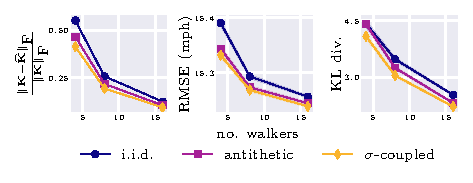
\includegraphics{images/traffic_graph_gps.pdf}
    \caption{Results for probabilistic traffic interpolation experiment. 
    Plots show the kernel approximation accuracy, test RMSE and KL divergence to the true posterior for graph kernels estimated using i.i.d., antithetic and $\sigma$-coupled GRFs.
    Lower is better.
    $\sigma$-coupling gives the best results for approximate inference.
    One standard error over random draws of walkers is shaded.}
    \label{fig:traffic}
\end{figure}